% I seguenti commenti speciali impostano:
% 1. thesis.tex come documento principale;
% 2. il controllo ortografico italiano per l'editor.

% !TEX root = thesis.tex
% !TEX spellcheck = it-IT

\documentclass[italian, noexaminfo]{sapthesis}  % italiano come linguaggio base di Sapthesis, che imposta il liunguaggio dei titoli, capitoli, ecc in italiano.

%**************************************************************
% Importazione package
%************************************************************** 

\usepackage[italian]{babel}     % per scrivere in italiano   
\usepackage{multicol}           % per la suddivisione dei fogli in due colonne
\usepackage{hyperref}   	    % collegamenti ipertestsuali
\usepackage{microtype}          % rifinimenti tipografici
\usepackage{graphicx}           % inserimento immagini
\usepackage{float}              % per il corretto posizionamento di tabelle, immagini
\usepackage{paralist}
\usepackage{multirow}
\usepackage{booktabs}
\usepackage{enumitem}           % enumerate con indent custom
\usepackage{amsfonts}           % font matematici come \mathbb

\setlength{\columnsep}{1.2cm}

\title{Applicazione di tecniche di machine learning ai log degli 
        accessi della piattaforma Infostud per analisi e predizione 
        di anomalie}
\author{Anthony Di Pietro}
\IDnumber{1960447}
\course{Informatica}
\courseorganizer{Ingegneria dell'informazione, informatica e statistica}
\AcademicYear{2022/2023}
\advisor{Prof. Tolomei Gabriele}
\coadvisor{Prof. Panizzi Emanuele}
\copyyear{2023}
\authoremail{dipietro.1960447@studenti.uniroma1.it}

\begin{document}    
    \frontmatter

    \maketitle
    % !TEX root = ../thesis.tex
    
%**************************************************************
% Dedica
%**************************************************************

\dedication{Dedicato a \\Martina
    \vspace*{12cm}
    \begin{center}
        Quando piove sotto gli alberi non piove\\
        Quando fuori smette è sotto gli alberi che piove \\
        \medskip --- Tarek Iurcich
    \end{center}
}                              % dedica
    % !TEX root = ../thesis.tex
    
%**************************************************************
% Abstract
%**************************************************************

\begin{abstract}
    Le serie temporali multivariate rappresentano un campo di studio 
    di notevole rilevanza in svariati sistemi distribuiti in tutto 
    il mondo. In un certo senso, queste serie di dati delineano 
    il ciclo di vita del sistema. Si può dunque dedurre che 
    attraverso le serie temporali vengono modellati sia i periodi 
    in cui il sistema funziona normalmente, che dualmente i periodi
    più "anomali".

    L'analisi delle serie temporali multivariate, con l'obiettivo 
    di identificare e predire anomalie, non deve solamente tener 
    conto della dipendenza temporale, un problema già complesso di 
    per sé, ma deve anche considerare la correlazione tra i vari 
    segnali all'interno del sistema. 
    
    Nel corso degli anni, diversi algoritmi sono stati impiegati 
    per l'analisi di anomalie nelle serie temporali, tra cui 
    SVM\cite{ocsvm} (Support Vector Machine), ma con risultati insoddisfacenti.
    Questi modelli presentano una limitazione fondamentale 
    che compromette la loro efficacia nell'analisi delle serie 
    temporali: la loro incapacità di catturare la correlazione 
    temporale, una caratteristica essenziale per condurre 
    un'analisi accurata di tali serie. Modelli come ARMA\cite{arma}, invece,
    riescono a catturare la dipendenza temporale, ma sono per natura 
    monovariati, per cui non sono in grado di osservare l'intercorrelazione 
    dei segnali.

    La ricerca sull'individuazione delle anomalie, negli anni recenti, ha fatto 
    molti passi avanti. Algoritmi come Telemanom\cite{telemanom} vengono applicati 
    a sistemi reali, complessi e delicati con ottimi risultati.
    
    L'anno 2019 è stato di particolare interesse per l'analisi di anomalie
    di serie temporali multivariate, grazie alla pubblicazione 
    dell'articolo scientifico sul modello Multi-Scale Convolutional 
    Recurrent Encoder-Decoder\cite{mscred} (MSCRED).
    MSCRED affronta la necessità di misurare non solo 
    l'intercorrelazione tra i dati, ma anche la loro dipendenza 
    temporale.

    In questa tesi, verrà applicato MSCRED su un sistema reale che riveste un ruolo di 
    straordinaria importanza per tutta la comunità accademica della Sapienza: il 
    prezioso dataset di Infostud, piattaforma che rappresenta una risorsa inestimabile 
    per la nostra istituzione, essendo un punto di riferimento fondamentale per 
    le attività accademiche e amministrative. 
    
    Verranno valutate le prestazioni di MSCRED, confrontando i risultati ottenuti 
    con quelli generati dagli algoritmi OC-SVM, ARMA e Telemanom. È importante 
    sottolineare che MSCRED, grazie alla sua capacità di analisi delle serie 
    temporali multivariate, si prevede porterà a risultati notevolmente 
    superiori rispetto agli altri modelli. Questa analisi rappresenta 
    un passo significativo verso un possibile miglioramento delle operazioni e 
    dell'efficienza del sistema Infostud.
\end{abstract}                            % abstract
    % !TEX root = ../thesis.tex
    
%**************************************************************
% Ringrazsiamenti
%**************************************************************

\begin{acknowledgments}
    Desidero esprimere la mia profonda gratitudine al \textbf{Professor 
    Gabriele Tolomei}, che mi ha concesso l'opportunità di 
    immergermi nell'ambito della scienza dei dati a livello pratico. 
    La data science rappresenta una disciplina informatica per la 
    quale ho sempre nutrito una profonda passione, e non potevo davvero 
    chiedere di meglio.

    Non posso non menzionare il contributo fondamentale del \textbf{Professor 
    Emanuele Panizzi} e del \textbf{Dottor Enrico Bassetti}, che hanno 
    generosamente messo a mia disposizione il dataset relativo ai log 
    degli accessi di Infostud, consentendomi così di applicare modelli 
    su un set di dati concreto ed estremamente interessante.
    
    Infine, ma non meno importante, desidero esprimere 
    la mia riconoscenza al collega \textbf{Edoardo Gabrielli}, il quale mi ha 
    guidato e sostenuto in tutto il corso del mio tirocinio, fornendomi
    preziosi consigli e un costante supporto morale. La sua preziosa
    assistenza è stata fondamentale per il mio percorso di ricerca e 
    studio.
\end{acknowledgments}                     % ringraziamenti

    \tableofcontents
    \mainmatter
    % !TEX root = ../thesis.tex
    
%**************************************************************
% Introduzione
%**************************************************************

\chapter{Introduzione: anomaly detection} \label{cap:intro}
    I sistemi complessi sono ubiqui nell'industria moderna e nei servizi dai quali tutti noi traiamo vantaggio 
    quotidianamente. La complessità di 
    tali sistemi i quali, di norma, prevedono la ricezione e l'elaborazione di un certo input, adempiono a task 
    potenzialmente ortogonali e, spesso, processano dati potenzialmente eterogenei ricavati dalla grande 
    quantità di dispositivi e sensori connessi, suscita inquietudini su potenziali anomalie che possono avere
    fonti e natura varie; che sia per il malfunzionamento di uno dei componenti propri del sistema o 
    dei suoi dispositivi connessi, o deviazioni nella natura del dominio del sistema. 
    
    In linea generale, i dati estratti delineano il ciclo di vita del sistema ed è cruciale identificare tempestivamente
    qualsiasi irregolarità per identificare la radice del problema e 
    contestualmente prevenire o minimizzare perdite; perdite la cui rilevanza può essere di natura finanziaria, 
    dove pochi minuti di malfunzionamenti potrebbero tradursi in danni economici di cifre a sei o sette zeri. In sistemi ancora 
    più delicati, come quelli presenti su un aereomobile, tali perdite potrebbero persino mettere a 
    rischio la vita dei passeggeri e dell'equipaggio di volo.

    Di solito, le serie temporali multivariate presentano un certo grado di rumore nelle applicazioni del 
    mondo reale. Pertanto, i modelli concepiti per affrontare il problema della rilevazione di anomalie devono 
    essere sviluppati prendendo in seno tale eventualità. Sarebbe auspicabile che gli algoritmi di 
    detection potessero definire una misura numerica dei punti anomali basata sulla gravità degli eventi 
    che hanno originato tali anomalie. In questo modo, le aziende e gli operatori potrebbero agire in modo 
    relativo e dinamico per risolvere il problema e, potenzialmente, prevenire l'insorgere di un'anomalia 
    prima che essa si manifesti.

    I ricercatori hanno esplorato e implementato modelli incentrati sui dati per l'identificazione e l'analisi 
    di anomalie e negli ultimi anni la questione, grazie a tecniche avanzate di machine learning e deep 
    learning e amplificata dalla moltitudine di dati collezionati, è diventata sempre più saliente. 


    Le anomalie possono essere suddivise in tre macrocategorie:
    \begin{enumerate}
        \item \textbf{Anomalie a punto} che corrispondono a singoli dati nel tempo considerati "outlier"
            poiché si discostano significativamente dal comportamento standard del resto del dataset. 
            La \hyperref[fig:point-anomaly]{Figura 1.1} 
            illustra un esempio di un dataset in cui si è verificata un'anomalia di tipo puntuale. Possiamo
            notare che un'osservazione, quella evidenziata in rosso, ha un valore notevolmente superiore 
            rispetto al resto del dataset.
            \begin{figure*}[htb]
                \centering
                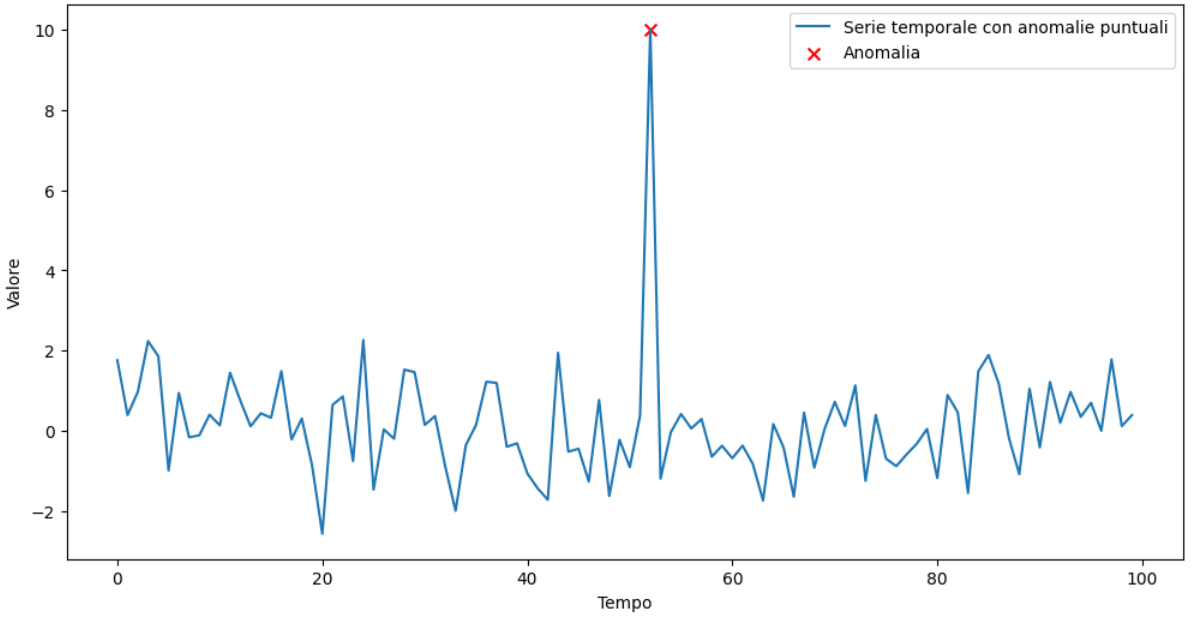
\includegraphics[width=0.6\textwidth]{./input/chapters/figs/point-anomaly.png}
                \caption{Dataset sintetico con anomalia a punto. Il dataset, ad esempio, potrebbe rappresentare il grado 
                di performance di un atleta in un intervallo di cento giorni. L'anomalia puntuale potrebbe indicare un 
                errore nell'inserimento dei dati.}
                \label{fig:point-anomaly}
            \end{figure*}
        \item \textbf{Anomalie contestuali} le quali rappresentano punti, o sequenze di punti, differenti 
        o distanti dal resto del dataset ma solo se presi in considerazione in un contesto specifico, che sia
        spaziale o temporale. 
        La \hyperref[fig:contextual-anomaly]{Figura 1.2.} fornisce un esempio di due anomalie di un dataset 
        sintetico che rappresenta l'indice di temperatura in una finestra temporale lunga due anni. 
        Questi punti, quando considerati nel loro contesto temporale, risultano essere anomalie; 
        tuttavia se analizzassimo complessivamente il dataset senza tener conto dell'ordinamento temporale, 
        essi non sembrerebbero affatto fuori dall'ordinario.

        \begin{figure}[H]
            \centering
            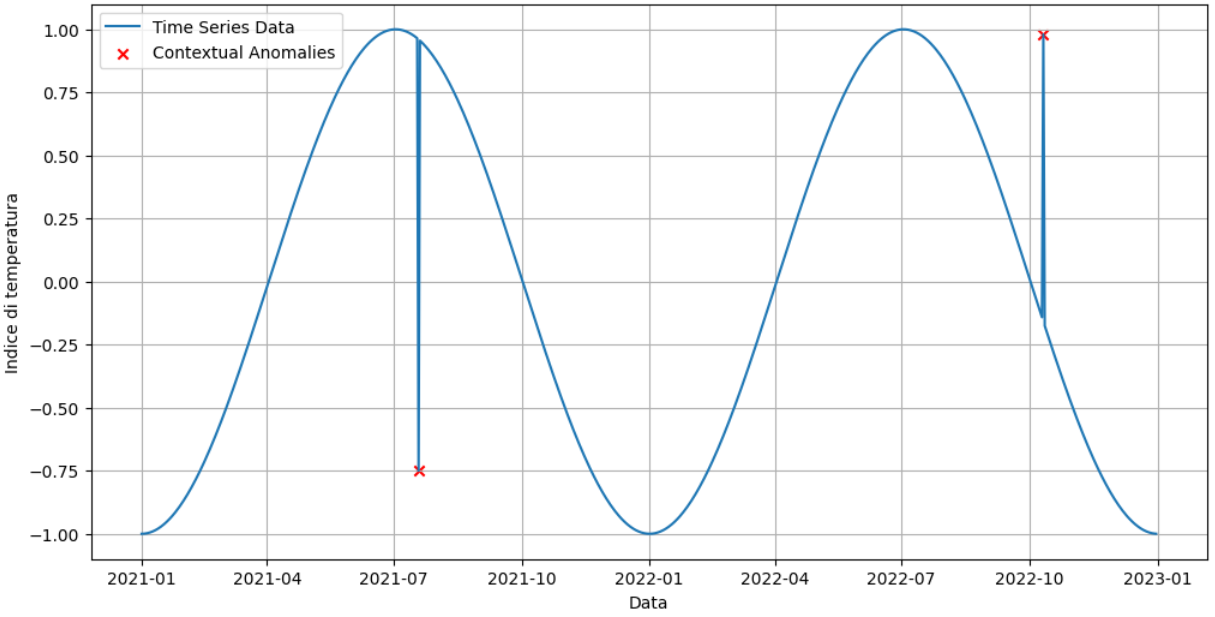
\includegraphics[width=0.6\textwidth]{./input/chapters/figs/contextual-anomaly.png}
            \caption{Dataset sintetico con anomalie contestuali. Il dataset rappresenta un indice di temperatura
            lungo due anni. Le anomalie contestuali nell'esempio registrano un grado di temperatura molto più bassa della norma a luglio e 
            una temperatura molto più alta a ottobre.} 
            \label{fig:contextual-anomaly}
        \end{figure}     
    
        \item \textbf{Anomalie collettive} si riferiscono a modelli che coinvolgono insiemi di osservazioni divergenti 
        rispetto al resto del dataset. Per esempio, la \hyperref[fig:collective-anomaly]{Figura 1.3.} presenta una 
        serie temporale contenente una sottoserie temporale evidenziata in rosso, la quale si differenzia dalle 
        altre sottoserie. In un contesto ipotetico, questa situazione potrebbe rappresentare un contatore bloccato 
        con problemi nell'aggiornamento dei dati.

        \begin{figure}[H]
            \centering
            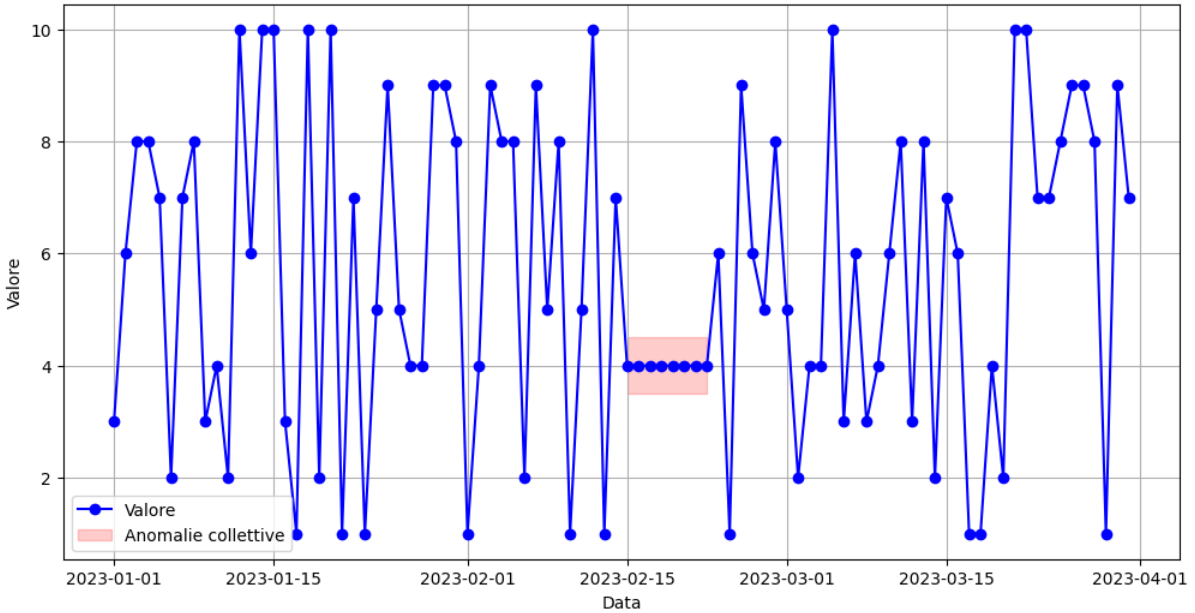
\includegraphics[width=0.6\textwidth]{./input/chapters/figs/collective-anomalies.png}
            \caption{Dataset sintetico con anomalie collettive. Il dataset può essere visto come la rappresentazione di un contatore il quale, 
            nel momento in cui avvengono le anomalie collettive, rimane bloccato.}
            \label{fig:collective-anomaly}
        \end{figure}   
    \end{enumerate}
    L'individuazione delle anomalie nell'ambito del machine learning, come chiaramente 
    illustrato nei precedenti esempi, è influenzata da una serie di fattori.
    Se tali fattori non vengono considerati in fase iniziale, potrebbero condurre a un'analisi poco accurata o addirittura errata. 
    Come si sottolinea in modo particolare nella \hyperref[fig:contextual-anomaly]{Figura 1.2.} e nella 
    \hyperref[fig:collective-anomaly]{Figura 1.3.}, i modelli devono tener conto della dipendenza temporale 
    delle osservazioni. Nella \hyperref[fig:temporal-dependency]{Figura 1.4.} è mostrato un semplice esempio
    di dipendenza temporale: il prezzo delle azioni a tempo $t$ dipende dal prezzo al tempo $t-1$ e influenza 
    il prezzo del tempo $t+1$. I modelli, inoltre, devono essere sviluppati sulla base che i dati su cui saranno addestrati 
    possono vivere in contesti multivariati; è bene che gli algoritmi osservino i vari segnali di un dataset 
    prendendo in considerazione la loro correlazione.

\begin{figure}[H]
    \centering
    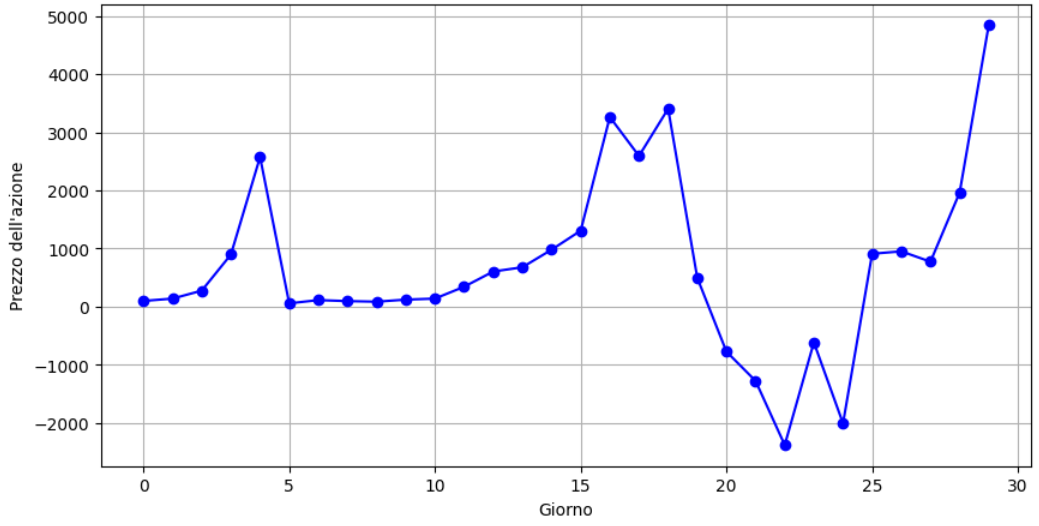
\includegraphics[width=0.6\textwidth]{./input/chapters/figs/temporal-dependency.png}
    \caption{Dataset sintetico con dipendenza temporale rappresentante un prezzo di un'azione nel tempo. La dipendenza temporale è dovuta
    al fatto che il prezzo in un generico tempo $t$ influisce sul prezzo al tempo $t+1$.}
    \label{fig:temporal-dependency}
\end{figure}    

    Il problema della rilevazione delle anomalie può essere affrontato mediante un approccio supervisionato, 
    il cui obiettivo è classificare in modo arbitrario le osservazioni anomale da quelle non anomale. 
    La peculiarità di questo approccio è che le anomalie, per essere definite tali, rappresentano una minoranza 
    all'interno del dataset.

    Un approccio non supervisionato è preferibile per il problema dell'individuazione delle anomalie. Algoritmi 
    diversi che utilizzano metodologie varie, come quella statistica con Auto Regressive Moving Average\cite{arma} (ARMA) e quella del machine learning per algoritmi come 
    One-Class Support Vector Machine\cite{ocsvm} (OC-SVM), o il deep learning con Telemanom\cite{telemanom} e MSCRED\cite{mscred}
    cercano di discriminare le anomalie dalle osservazioni non anomale senza la necessità di disporre
    delle etichette ground-truth, ma basandosi esclusivamente sull'analisi della serie 
    temporale di interesse. Questo metodo, oltre a essere più idoneo, semplifica notevolmente 
    la fase di preparazione dei dati escludendo la costruzione delle etichette.

    La tesi è strutturata in cinque capitoli.
    \begin{enumerate}
        \item Nel primo capitolo, quello corrente, viene fatta una piccola paronamica riguardo al problema dell'analisi delle anomalie.
        \item Nel secondo capitolo vengono osservate le metriche e la finestra temporale del dataset di Infostud su cui si 
                sono svolti gli esperimenti e vengono giustificate le ragioni per cui è stato scelto quel dataset in particolare.
        \item Il terzo capitolo illustra le varie metodologie applicate per la risoluzione del problema dell'anomaly detection
                al prezioso dataset di Infostud, per auspicabilmente risolvere e tracciare anomalie ai fini del miglioramento 
                della piattaforma più cara a tutta la comunità accademica de La Sapienza. Verranno illustrate le applicazioni di 
                tre approcci diversi: statistico, machine learning e deep learning.
        \item Nel capitolo quattro verranno presentate le metriche di valutazione ai fini di giudicare le performance delle soluzioni 
                dei vari algoritmi. Nello stesso capitolo, verranno anche mostrati i risultati dei vari modelli utilizzati.           
        \item Nell'ultimo capitolo sono riportate e confrontate le conclusioni dei modelli analizzati.           
    \end{enumerate}


    Tutti gli esperimenti citati in questa relazione sono disponibili su 
    GitHub\footnote{https://github.com/Pikarz/tirocinio\_infostud} al link riportato a piè di pagina.     % introduzione
    % !TEX root = ../thesis.tex
    
%**************************************************************
% Dataset
%**************************************************************

\chapter{Il dataset di Infostud} \label{cap2}
    Il dataset preso in analisi, relativo a Infostud, gentilmente fornito dal Professor E. Panizzi e dal Dottor 
    E. Bassetti, riveste un'enorme importanza per l'intera comunità accademica de La Sapienza.

    Il dataset rappresenta svariate 
    metriche raccolte dalle piattaforme InfoSapienza e dalle richieste inoltrate attraverso 
    Infostud alla piattaforma esterna GOMP. I dati vengono utilizzati ai fini di monitoraggio e 
    sono raccolti attraverso il software Prometheus. 
    
    \paragraph{Il dataset in dettaglio} La finestra temporale di osservazione dei dati su cui si sono 
    svolti gli studi è lunga poco più di quattro anni, da gennaio 2019 a febbraio 2023, con una frequenza di campionamento di circa 
    una misurazione ogni 15 secondi per le metriche più dense. Il Dottor Bassetti ha anche tenuto traccia di 
    una buona fetta di anomalie effettivamente verificatesi su Infostud nella stessa finestra temporale, 
    garantendo quindi un prezioso ambiente supervised che ha consentito di avere riscontri numerici sulle 
    performance dei modelli in analisi.


    Nel complesso, il dataset è composto da settecentocinquanta file; tali file sono suddivisi per piattaforma, 
    ovvero GOMP e InfoSapienza, e tipologia di metrica. Ciascun file rappresenta 
    circa trenta giorni di osservazioni. Ai fini dell'analisi effettuata con i modelli è stata presa
    in considerazione la parte dei dati strettamente appartenenti a Infostud. 
    
    Di seguito sono riportate in dettaglio le informazioni delle varie tipologie di metriche osservate lato 
    InfoSapienza:
    \begin{enumerate}[leftmargin=14pt]
        \item \texttt{http\_responses}  Contatore di richieste HTTP in cui ogni segnale rappresenta un codice di stato 
                                            riscontrato dalla richiesta. 
                                            Ad esempio, il segnale 200 rappresenta le richieste elaborate con 
                                            successo (codice di stato OK), mentre 401 rappresenta un errore e 
                                            comunica che l'autenticazione HTTP non è riuscita (codice di stato 
                                            Unauthorized). Il contatore è monotonico salvo eventuali reset 
                                            a cadenza non regolare.
        \item \texttt{requests\_total}  Contatore delle richieste totali effettuate a InfoSapienza. Anche qui, il contatore 
                                            è monotonico tra due reset.
        \item \texttt{phoenixws\_requests\_delay\_bucket} 
                                            Ogni segnale rappresenta un bucket a cui è associato un certo valore $le$ (\emph{less or equal}).
                                            Il bucket accumula le latenze delle richieste ai servizi InfoSapienza. 
                                            Ad esempio, se al tempo $t$ avvengono $x$ richieste a $y$ servizi InfoSapienza
                                            e tali richieste vengono risposte con latenza minore o uguale al valore $le$, 
                                            allora tale bucket avrà un valore pari a $x$. È bene 
                                            notare che i bucket non sono disgiunti e il numero di segnali non è uniforme 
                                            tra i file. I segnali, in generale, sono sull'ordine delle centinaia.
        \item \texttt{phoenixws\_requests\_delay\_count}
                                            Contatore di richieste processate a servizi. Ogni segnale è un tipo di servizio
                                            diverso come, ad esempio, la ricerca degli esami o il login. In genere, questi file 
                                            contengono diciotto segnali diversi.
        \item \texttt{phoenixws\_requests\_delay\_sum}
                                            Somma delle latenze delle richieste a servizi. I servizi osservati sono gli 
                                            stessi dei file di tipologia \texttt{phoenixws\_requests\_delay\_count}.                                
    \end{enumerate}

In \hyperref[tab:infosapienza-metrics]{Tabella 2.1.} è illustrato un riassunto delle varie metriche del dataset.
 \begin{table}[H]
    \centering
    \caption{Tipologie di metriche lato Infosapienza.}
    \begin{tabular}{p{0.45\linewidth}p{0.5\linewidth}}
        \toprule
        \textbf{Metrica} & \textbf{Dettagli} \\
        \toprule
        \texttt{http\_responses} & Contatore in cui ogni segnale è associato a un tipo di richiesta HTTP. \\
        \midrule
        \texttt{request\_total} & Contatore totale delle richieste HTTP. \\
        \midrule
        \texttt{phoenixws\_requests\_delay\_bucket} & Insieme di bucket. A ogni bucket è associato un valore $le$ e tale bucket accumula le latenze inferiori o uguali a $le$. \\
        \midrule
        \texttt{phoenixws\_requests\_delay\_count} & Contatore di richieste processate a servizi. Ogni segnale rappresenta un tipo di servizio. \\
        \midrule
        \texttt{phoenixws\_requests\_delay\_sum} & Somma delle latenze delle richieste a servizi. Ogni segnale rappresenta un tipo di servizio. \\
        \bottomrule
    \end{tabular}
    \label{tab:infosapienza-metrics}
\end{table}

    \paragraph{Trasformazione delle etichette}
    Le etichette sono state provvedute sottoforma di file. Ogni file rappresenta 
    un certo intervallo in cui si è verificata un'anomalia. I file hanno anche altre informazioni riportate nella 
    \hyperref[tab:info-labels]{Tabella 2.2}

    Poiché una certa fetta di dataset può contenere più punti all'interno dei vari intervalli di tutti i file delle 
    etichette, è stato creato un dataset binario che mappa un certo timestamp del dataset a un valore di verità: vero 
    se quel timestamp è all'interno di uno degli intervalli dei file delle etichette, ovvero quel timestamp è 
    all'interno di un periodo anomalo del sistema, falso altrimenti.

\begin{table}[H]
    \centering
    \caption{Le informazioni dei file delle etichette.}
    \begin{tabular}{p{0.45\linewidth}p{0.5\linewidth}}
        \toprule
        \textbf{Informazione} & \textbf{Significato} \\
        \toprule
        \texttt{Title} & Tipo di anomalia, ad esempio `Irrangiugibilità Infostud'. \\
        \midrule
        \texttt{Date} & Data di inizio dell'anomalia. \\
        \midrule
        \texttt{resolved} & Valore binario che indica se l'anomalia è stata risolta o no. \\
        \midrule
        \texttt{resolvedWhen} & Data di termine dell'anomalia. \\
        \midrule
        \texttt{Severity} & Grado di severità del problema. \\
        \midrule
        \texttt{affected} & Servizi o insiemi di servizi che hanno subito malfunzionamenti \\
        \bottomrule
    \end{tabular}
    \label{tab:info-labels}
\end{table}

    \paragraph{La scelta del tipo di dataset} \label{cap2:hypothesis} I primi esperimenti si sono basati sui file di tipologia 
    \texttt{http\_responses}. Questi esperimenti non hanno portato a soluzioni di particolare rilievo per 
    ciascun modello applicato, ma sono stati fondamentali per familiarizzare con il dataset. La 
    seconda trance di esperimenti si è focalizzata su tre tipologie di file diversi: 
    \texttt{phoenixws\_requests\_delay\_bucket}, \texttt{phoenixws\_requests\_delay\_count} e 
    \texttt{phoenixws\_requests\_delay\_sum}. È banale che i bucket, essendo la categoria predominante nel 
    dataset, hanno comportato un'elevata esposizione dei modelli a tali dati rispetto che alle altre metriche.
    Difatti gli esperimenti che si sono basati su questi dati non hanno portato soluzioni interessanti. 


    Dopo questi tentativi iniziali, che hanno comunque contribuito a una migliore comprensione dei dati e dei 
    modelli, è stata presa la decisione, in collaborazione con il relatore, il Professore G. Tolomei, di 
    concentrarsi sugli esperimenti successivi utilizzando un dataset ibrido: abbiamo osservato che, 
    avendo a disposizione la somma delle latenze fatte ai servizi di Infosapienza 
    \texttt{phoenixws\_requests\_delay\_sum} e il relativo contatore \texttt{phoenixws\_requests\_delay\_count},
    era possibile creare il dataset che rappresentasse la latenza media di ogni richiesta per ogni servizio. 
    Si prevedeva che questo approccio potesse portare a risultati migliori nell'analisi e nell'individuazione di anomalie.

    
    \paragraph{La scelta della finestra temporale} In virtù delle etichette e del nuovo dataset, dopo un'attenta analisi, 
    gli esperimenti successivi si sono focalizzati su diverse fette temporali che hanno dovuto soddisfare alcune proprietà
    chiave:
    \begin{enumerate}
        \item i dati devono rientrare in una finestra di osservazione all'interno di quella delle etichette, 
              le quali non sono disponibili per tutto il dataset;
        \item la percentuale di anomalie riscontrate deve essere intorno al $5\%$ per garantire al modello di essere addestrato 
              con un numero sufficiente di anomalie, ma non troppe per non rischiare che esso classifichi fluttuazioni anomale 
              come normali;
        \item la suddivisione del dataset in insiemi di training, validazione e test deve garantire a tutti e tre i 
              sottoinsiemi di contenere anomalie ed è auspicabile che la percentuale di anomalie sia quantomeno 
              simile per tutti e tre i sottoinsiemi di dati;
        \item i dati devono essere poco vuoti, ovvero non devono contenere troppi valori nulli per 
              preservare il più possibile l'integrità originale dei dati. Questo perché i modelli, per essere addestrati, 
              necessitano di un dataset privo di valori nulli i quali, purtroppo, sono inevitabilmente presenti;
        \item per limiti computazionali i dati non devono contenere troppi punti, ma al più devono basarsi su tre mesi 
              di osservazioni.
    \end{enumerate}
    
\begin{table}[H]
    \centering
    \caption{Riassunto delle proprietà del dataset su cui verranno basati gli esperimenti.}
    \begin{tabular}{p{0.55\linewidth}p{0.4\linewidth}}
        \toprule
        \textbf{Proprietà} & \textbf{Motivazione}\\
        \toprule
        L'intera finestra temporale delle osservazioni prese in considerazione deve essere inclusa in quella delle 
        etichette. & Consente di avere riscontri numerici sulle performance.  \\
        \midrule
        Percentuale di anomalie $\approx 5\%$. & Le anomalie devono essere presenti e non devono occupare una grande parte di dataset.  \\
        \midrule
        La percentuale di anomalie negli insiemi di training, validation e test deve essere simile e sempre maggiore di zero. 
        & I tre insiemi devono osservare una percentuale simile di anomalie.\\
        \midrule
        I dati non devono contenere molti valori nulli. & Mantiene l'integrità del dataset. \\
        \midrule
        Al massimo tre mesi di osservazioni. & Per soddisfare limiti computazionali.\\
        \bottomrule
    \end{tabular}
    \label{tab:data-properties}
\end{table}

   \paragraph{Pre-processamento dei dati} Per la creazione del dataset delle latenze medie è necessaria una divisione 
   elemento per elemento tra i due dataset \texttt{phoenixws\_requests\_delay\_sum} e \texttt{phoenixws\_requests\_delay\_count}.

   Le proprietà da soddisfare, illustrate nella \hyperref[tab:data-properties]{Tabella 2.3.}, sono varie. Per composizione 
   del dataset, molto problematico è il punto in cui è espressa la necessità che il dataset preso in analisi non debba
   contenere molti valori nulli, e per far sì che venga rispettato è stato doveroso eliminare le righe e le 
   colonne più vuote dei dataset presi in considerazione. 

   I dataset più interessanti che hanno soddisfatto tali proprietà, in seno all'eliminazione delle righe e colonne più 
   vuote, sono tre le cui informazioni sono illustrate nella \hyperref[tab:data-info]{Tabella 2.4.}
    
    \begin{table}[H]
        \centering
        \caption{Statistiche del dataset suddiviso in finestre temporali.}
        \begin{tabular}{lccc}
            \toprule
            \textbf{Finestra temporale} & \textbf{Anomalie (\%)} & \textbf{Valori nulli (\%)}  \\
            \toprule
            8 agosto - 11 novembre 2019  & 6\%   & 15\% \\
            23 febbraio - 24 marzo 2020  & 2.1\% & 16\%  \\
            23 maggio - 22 giugno 2020   & 5.6\% & 14.5\%  \\
            \bottomrule
        \end{tabular}
        \label{tab:data-info}
    \end{table}

    Tali porzioni di dataset, purtroppo, come illustrato, ancora presentano valori nulli. Per poter permettere ai modelli
    di essere applicati, è necessario sostituire i valori nulli con un valore che si presti bene al problema. In questi studi,
    i valori nulli sono stati sostituiti con la media relativa a ogni segnale. 

    Gli esperimenti sono stati condotti principalmente utilizzando il dataset relativo 
    al periodo dal 23 maggio al 22 giugno 2020, ma tutti i modelli possono essere applicati in maniera analoga a tutti 
    i dataset menzionati, con l'adeguamento degli iperparametri. 
    
    Il dataset preso in analisi ha visto la rimozione di un circa un quarto delle righe e un terzo delle 
    colonne meno dense, da diciotto a dodici.

    \begin{figure}[H]
        \centering
        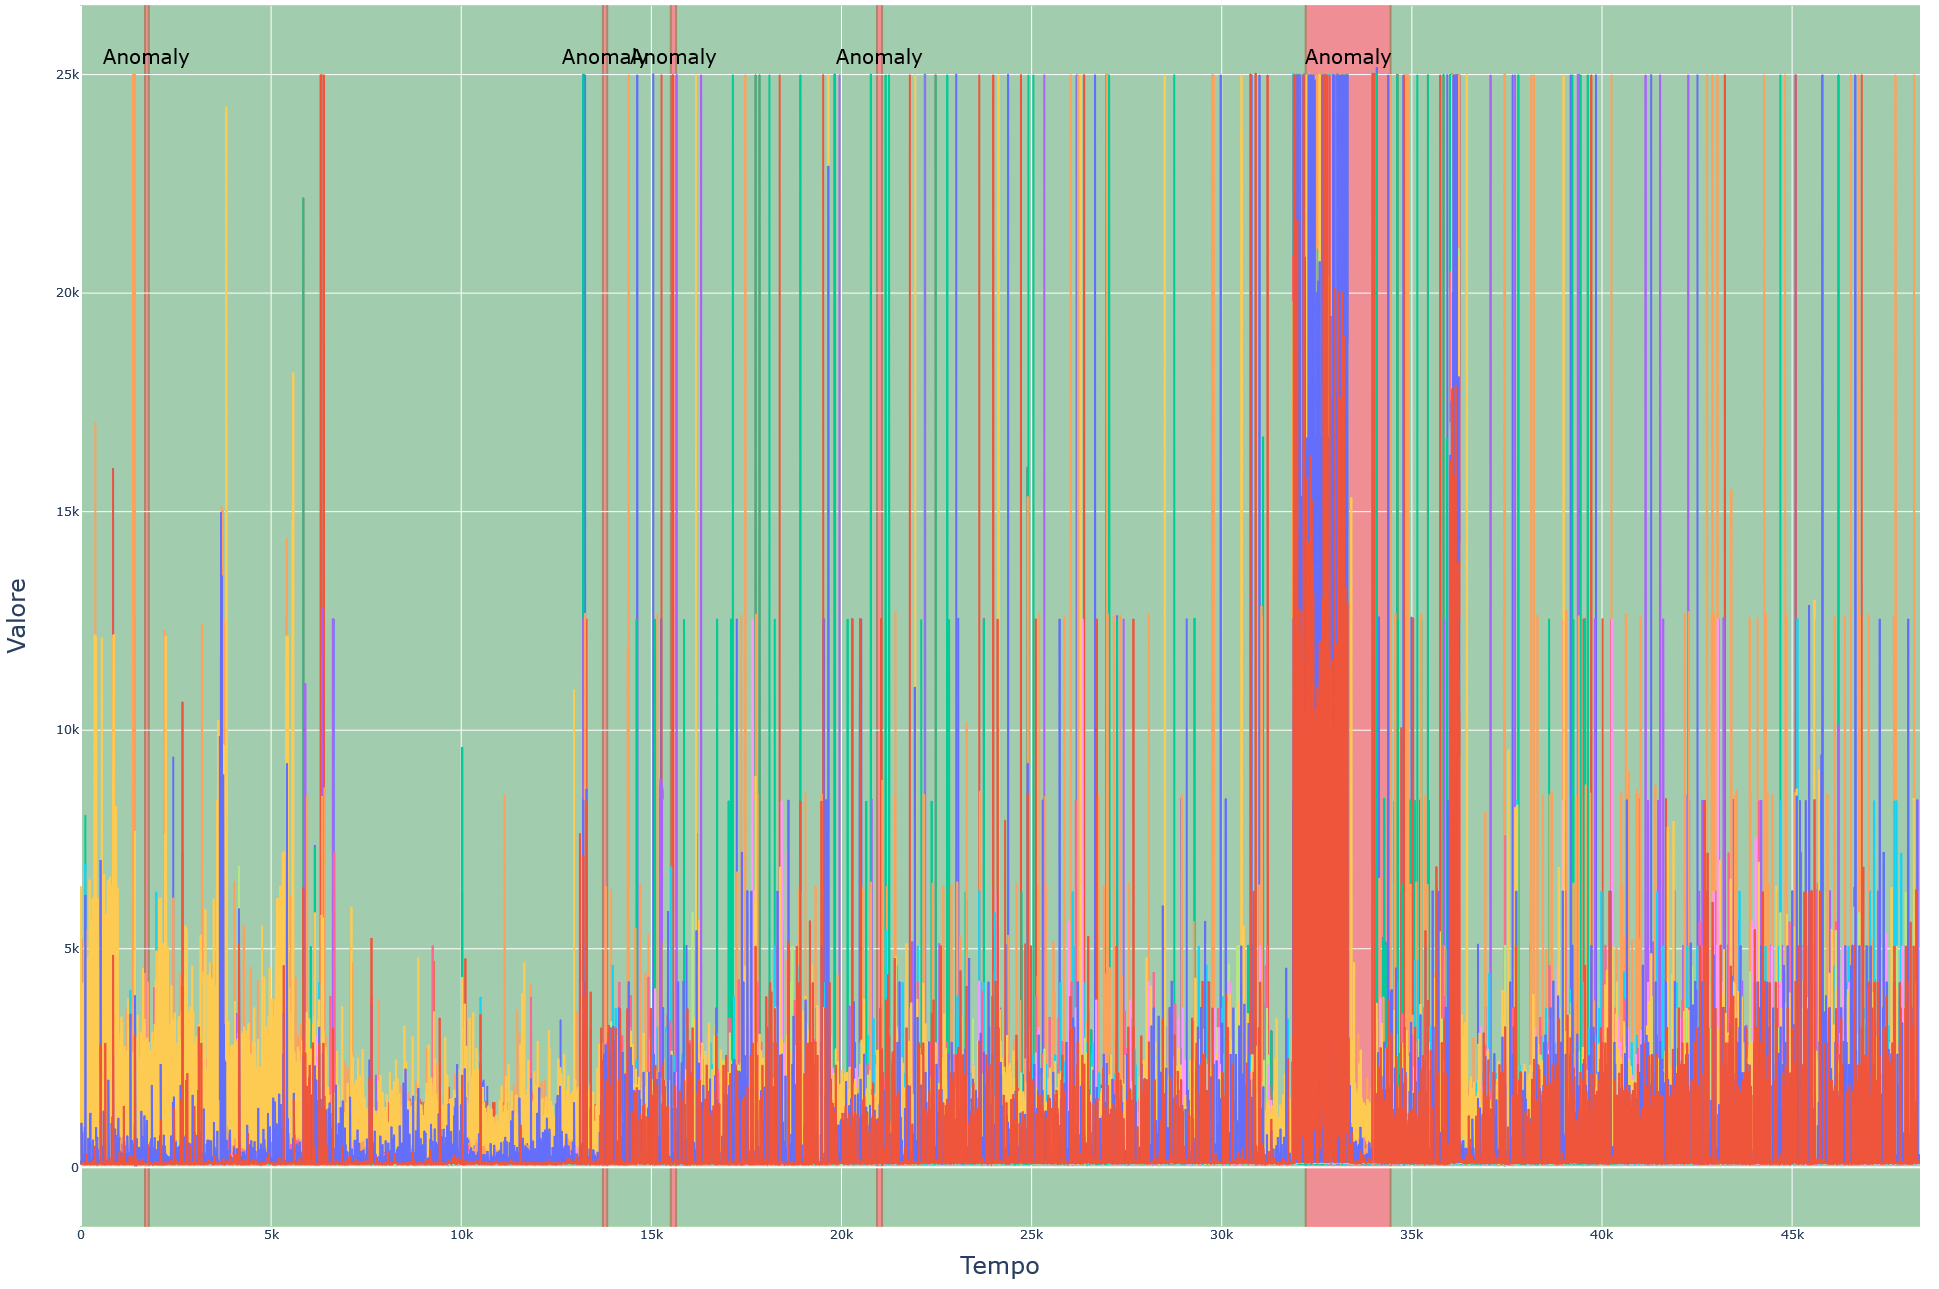
\includegraphics[width=0.6\textwidth]{./input/chapters/figs/plot-infostud.png}
        \caption{Dataset 23 maggio - 22 giugno 2020. Le bande rosse rappresentano le anomalie ground-truth, mentre quelle 
        verdi i periodi non anomali.}
        \label{fig:dataset-giugno}
    \end{figure}
    \begin{figure}[H]
        \centering
        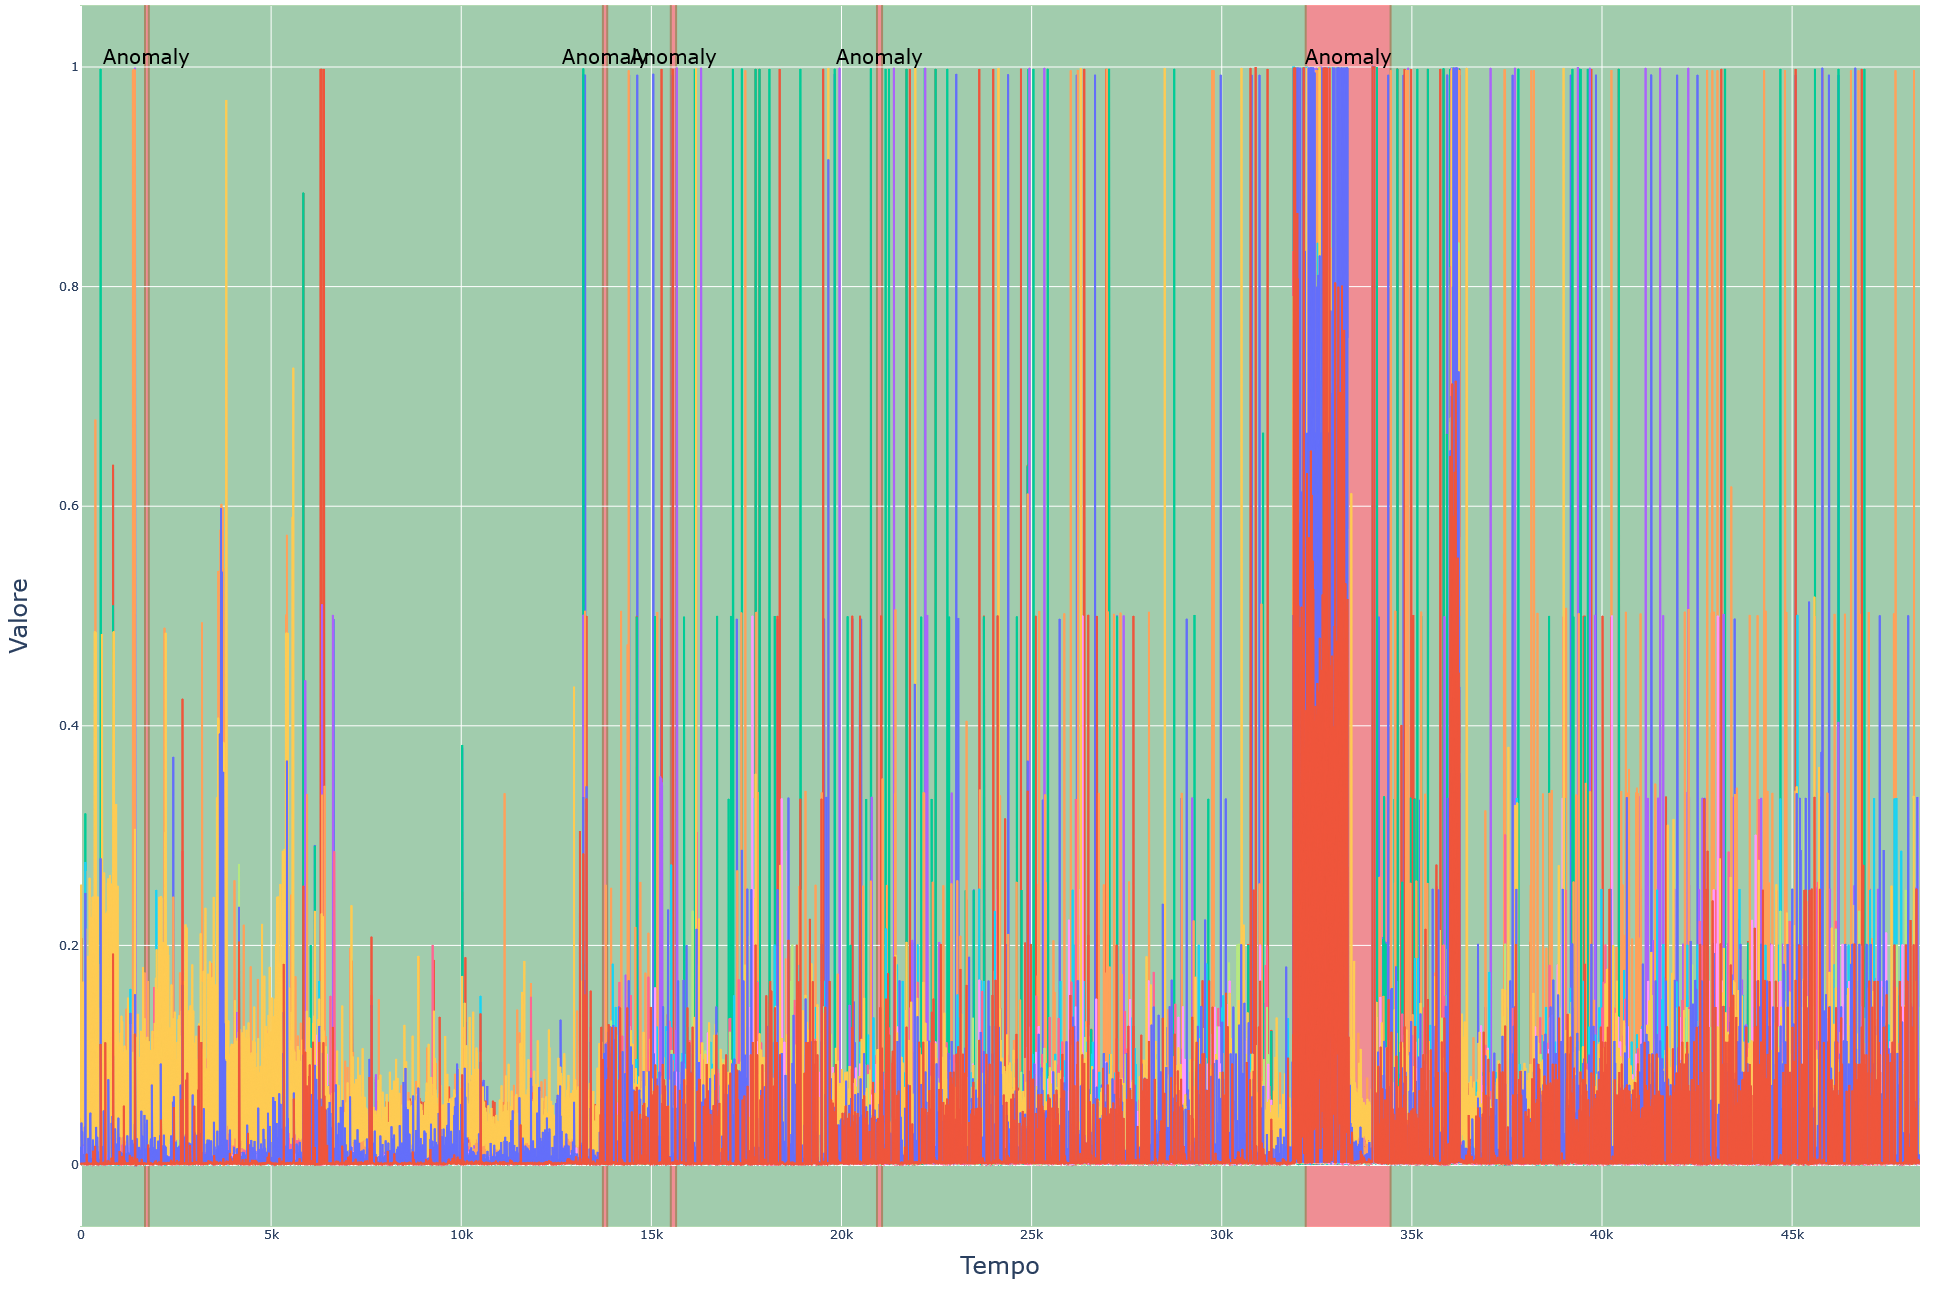
\includegraphics[width=0.6\textwidth]{./input/chapters/figs/plot-infostud-norm.png}
        \caption{Dataset 23 maggio - 22 giugno 2020 normalizzato senza valori vuoti. Le bande rosse rappresentano le anomalie ground-truth, mentre quelle 
        verdi i periodi non anomali.}
        \label{fig:dataset-giugno-norm}
    \end{figure}    
    

\paragraph{Visualizzazione del dataset preso in analisi}
    Il dataset su cui si basano gli esperimenti dei capitoli successivi è illustrato in 
    \hyperref[fig:dataset-giugno]{Figura 2.1.} 
    
    Possiamo osservare le anomalie che si sono presentate nelle aree in cui lo sfondo del grafico è rosso, 
    mentre le aree verdi rappresentano i periodi non anomali. È lampante che, nell'ultima anomalia, quella più 
    grande tra tutte le altre, i segnali sono molto più alti. Ci aspettiamo che un modello segnali quei periodi come 
    anomali. In \hyperref[fig:dataset-giugno-norm]{Figura 2.2.} possiamo osservare il dataset normalizzato con i 
    valori vuoti sostituiti dalla media relativa al segnale associato.

    È un privilegio poter affermare che l'applicazione di modelli metodologicamente diversi sul dataset di Infostud, indispensabile
    per la comunità Sapienza, rappresenta una straordinaria opportunità per gli studi intrapresi dal sottoscritto.          % dataset
    % !TEX root = ../../thesis.tex
    
%**************************************************************
% Methodology
%*************************************************************
\chapter{Metodologie di Analisi}
    Ai fini di valutare le performance delle soluzioni dei vari modelli applicati sul dataset che rappresenta la latenza media 
    delle richieste a servizi fatti a Infostud, viene proposto l'utilizzo di tre principali approcci metodologici per 
    l'analisi atta all'individuazione di anomalie nel dataset accademico. Le soluzioni verranno analizzate 
    in virtù delle etichette dapprima esistenti sul dataset:
    \begin{enumerate}
        \item \textbf{Approccio Statistico (Statistical-based):} L'approccio statistico si basa sulla tradizionale 
              statistica dei dati. In particolare ARMA\cite{arma}, il modello utilizzato per fare inferenza sulle anomalie 
              del prezioso dataset di Infostud, modella le relazioni temporali nei dati attraverso l'uso dell'autoregressione 
              e della media mobile, metodi adatti al fine di modellare le relazioni temporali nei dati; il modello 
              identifica tendenze e autocorrelazioni nelle metriche applicate.
        \item \textbf{Approccio di Apprendimento Automatico (Machine Learning-based):} Nell'ambito dell'apprendimento automatico, 
              è stato scelto l'approccio basato sulle Support Vector Machine (SVM). In particolare, la Support Vector 
              Machine a classe singola (OC-SVM\cite{ocsvm}), un algoritmo che si concentra sull'identificazione di 
              dati fuori dal normale comportamento in grado di tracciare confini decisionali creando due regioni che 
              discriminano, nel caso in questione, le anomalie dalle non anomalie.
        \item \textbf{Approccio di Apprendimento Profondo (Deep Learning-based):} L'apprendimento profondo è particolarmente 
              efficace nell'affrontare problemi di analisi di dati complessi, come le serie temporali.  
              Questo approccio vede applicati due modelli molto recenti: Telemanom\cite{telemanom} e Multi-Scale Convolutional 
              Recurrent Encoder-Decoder (MSCRED\cite{mscred}); entrambi sono modelli basati su reti neurali e sono 
              progettati con lo specifico obiettivo di individuazione delle anomalie in dati multivariati. 
    \end{enumerate}

    Ciascuno di questi approcci contribuisce in modo significativo all'analisi del dataset indispensabile per tutta 
    la comunità Sapienza, fornendo una varietà di strumenti e metodi per esplorare, valutare e interpretare le 
    informazioni contenute nei dati di Infostud. Nel corso di questo capitolo, verranno esaminate in dettaglio 
    le soluzioni di ciascuno dei modelli presi in considerazione.

    \section{Approccio Statistico (Statistical-based)}
        %**************************************************************
% ARMA
%**************************************************************

\subsection{Auto Regressive Moving Average}
    In questa sezione esploriamo l'uso del modello univariato ARMA\cite{arma} 
    (Auto Regressive Moving Average) come 
    modello di riferimento che adotta un approccio statistico per valutare e confrontare l'efficacia del modello MSCRED\cite{mscred}.
    La scelta del modello ARMA è stata motivata principalmente dalla sua 
    utilizzazione da parte dei ricercatori di MSCRED per valutare le prestazioni di quest'ultimo. In generale, 
    ARMA è un modello ben consolidato e ampiamente utilizzato nella letteratura grazie alla sua semplice 
    implementazione e intuitività.

    Tuttavia, la sua semplicità ha un costo: il modello non è in grado di catturare l'intercorrelazione 
    tra i segnali perché è monovariato per natura. 
    Nell'esperimento presentato, per adattarsi alla natura monovariata del modello, è stato selezionato il
    segnale meno vuoto dal dataset di Infostud descritto nel \hyperref[cap2]{Capitolo 2}, ovvero il segnale con
    il minor numero, solo dieci, di valori nulli, avendo quindi a disposizione un totale di 48327 osservazioni.
    Il segnale interessato rappresenta la latenza media delle richieste di login a InfoSapienza.


    \paragraph{Intuizione} ARMA, nelle serie temporali, è utilizzato principalmente per la previsione di dati, ma 
    può essere usato anche per la rilevazione di anomalie. In linea generale, data una previsione di ARMA, i punti 
    in cui la previsione si discosta maggiormente rispetto ai punti originali vengono considerati anomalie.

    Più in dettaglio, ARMA effettua una certa previsione $P$ basata sui dati di training. Tale previsione viene 
    confrontata con i valori ground-truth $G$ calcolando i residui $P-G$. Attraverso l'iperparametro $t$ 
    vengono calcolati i confini decisionali $c^-, c^+$. ogni punto $i$ è valutato come anomalia se $P_i-G_i \notin [c^-, c^+]$,
    e non è valutato come tale altrimenti. 
    I confini decisionali $c^-, c^+$ sono ottenuti come segue: siano $\mu$ la media dei valori dell'unico segnale
    del dataset e sia $\sigma$ la sua deviazione standard: $c^+ = \mu + t^*\cdot\sigma, c^- = \mu - t^*\cdot\sigma$



    \paragraph{Dataset}Il dataset di Infostud è stato suddiviso in tre insiemi: training, validation e
    test, con percentuali rispettivamente pari a $0.5, 0.182, 0.318$. Allo scopo di 
    garantire una distribuzione accettabile delle anomalie nei tre insiemi, questa suddivisione atipica è stata 
    necessaria a causa della natura delle anomalie nel dataset, che sono principalmente di tipo collettivo 
    e quindi vicine tra loro sia nel tempo che nello spazio.
    Nel dataset, come già annunciato, è stato preso in considerazione un solo segnale, quello che rappresenta 
    la latenza media delle richieste di login effettuate a InfoSapienza, i cui dieci punti originariamente nulli 
    sono stati rimossi.
    Nella \hyperref[tab:dataset-arma]{Tabella 3.1.} sono riportate le informazioni in dettaglio della suddivisione 
    del dataset e nella \hyperref[fig:dataset-arma]{Figura 3.1.} è illustrato il dataset.

    \begin{table}[H]
        \centering
        \caption{Statistiche dataset ARMA (latenza media delle richieste di login).}
        \begin{tabular}{lccc}
            \toprule
            \textbf{Dataset} & \textbf{Indice di split} & \textbf{\# punti} & \textbf{Anomalie (\%)} \\
            \midrule
            \textbf{Training} & 0.5 & 24163 & 2.01 \% \\
            \textbf{Validation} & 0.182 & 8796 & 8.59 \% \\
            \textbf{Testing} & 0.318 & 15368 & 9.59 \% \\
            \bottomrule
        \end{tabular}
        \label{tab:dataset-arma}
    \end{table}

    \begin{figure}[H]
        \centering
        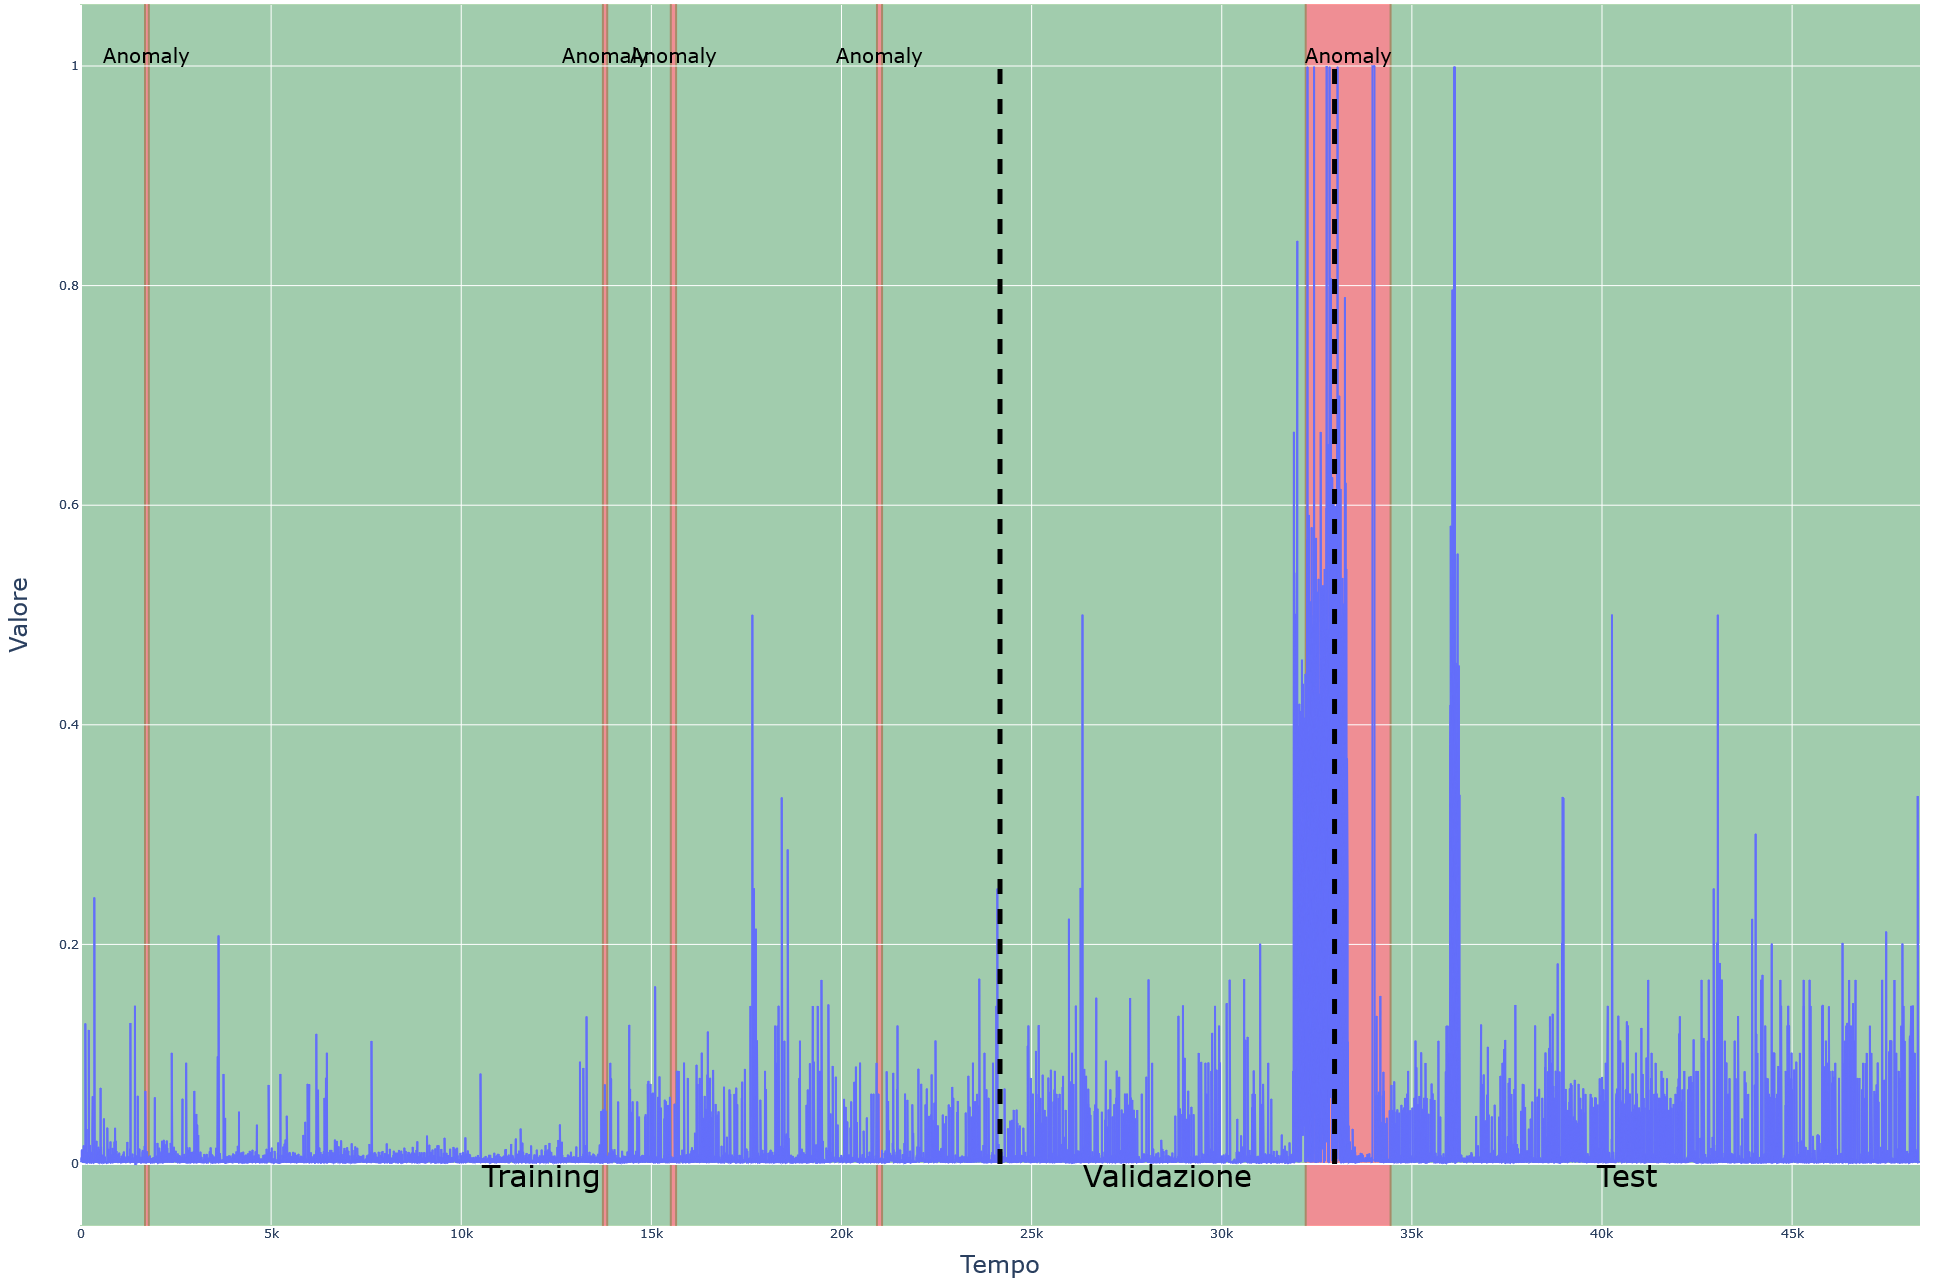
\includegraphics[width=0.6\textwidth]{./input/chapters/models/figs/arma-dataset.png}
        \caption{Dataset delle latenze medie alle richieste di login nel periodo 23 maggio - 22 giugno 2020. 
        Le bande rosse rappresentano le anomalie ground-truth, mentre quelle verdi i periodi non anomali. 
        Le linee tratteggiate delimitano il dataset di training da quello di validazione e quello di validazione dal test.}
        \label{fig:dataset-arma}
    \end{figure}

    \paragraph{Iperparametri} ARMA, in generale, presenta due iperparametri $p,q$. $p$ rappresenta l'ordine 
    dell'autoregressione nel modello ARMA. L'autoregressione si riferisce al fatto che il valore corrente 
    della serie temporale dipende dai valori passati della stessa serie temporale, in sintesi $p$ indica 
    quanti periodi temporali passati vengono utilizzati per predire il valore corrente ed è l'iperparametro 
    che fa sì che ARMA possa catturare le dipendenze temporali nella serie temporale. $q$, invece, 
    rappresenta l'ordine della media mobile nel modello. Essa indica che il valore della corrente serie 
    temporale dipende dai valori passati dei residui, ovvero degli errori previsionali, del modello stesso.
    Intuitivamente, $q$ indica quanti periodi temporali passati degli errori previsionali vengono utilizzati per 
    predire il valore corrente.

    Ai fini dell'anomaly detection, ARMA presenta anche un terzo iperparametro $t$ che, nel caso degli studi effettuati,
    è atto a creare i confini decisionali dei punti non anomali e, dualmente, anomali, definendo la sensibilità 
    del modello. 

    Per la scelta degli iperparametri è stata effettuata una grid-search di 30 epoche su $p$, $q$ e $t$  al fine di 
    individuare la combinazione che massimizzasse lo score F1, metrica illustrata nella \hyperref[f1-score]{Sottosezione 4.1.3}, 
    sul dataset di validation attraverso il training sul train set.

    Formalmente, siano $\mathbf{Tr}, \mathbf{Va}$ i dataset utilizzati per il training e
    per il validation rispettivamente, e sia $\text{ARMA}_\mathbf{X}^\mathbf{Y}$ un modello ARMA addestrato su 
    $\mathbf{X}$ che effettua previsioni nei punti $\mathbf{Y}$ e sia $T_{10}$ uno spazio lineare composto da 
    elementi equidistanti $t_i$ tali che $t_i \in [0.1, 5.0] \forall i \in [10]$:
    \begin{equation}
    \label{eq:arma-problem}
    \begin{aligned}
        & p^*, q^*, t^* = \max_{p, q, t} F1(\text{ARMA}_\mathbf{Tr}^\mathbf{Va}(p, q, t)) \\
        & \text{con il vincolo} \quad p, q \in [30], t \in T_{10}
    \end{aligned}
    \end{equation}


    \paragraph{Soluzione} \hyperref[eq:arma-problem]{L'equazione 3.1}  è stata soddisfatta dai seguenti:
    \begin{itemize}
        \item $p^* = 20$
        \item $q^* = 8$
        \item $t^* = 0.644$
    \end{itemize}

    Poiché l'insieme di validazione era necessario solo ai fini della ricerca degli iperparametri, è 
    stato successivamente accorpato al dataset di training. Dopo l'addestramento del modello sul nuovo dataset 
    con gli iperparametri che hanno generato una soluzione ottimale sul validation, sono state effettuate 
    le previsioni della serie temporale di test, mostrate nella \hyperref[fig:arma-sol]{Figura 3.2.}


    \begin{figure*}[h]
        \centering
        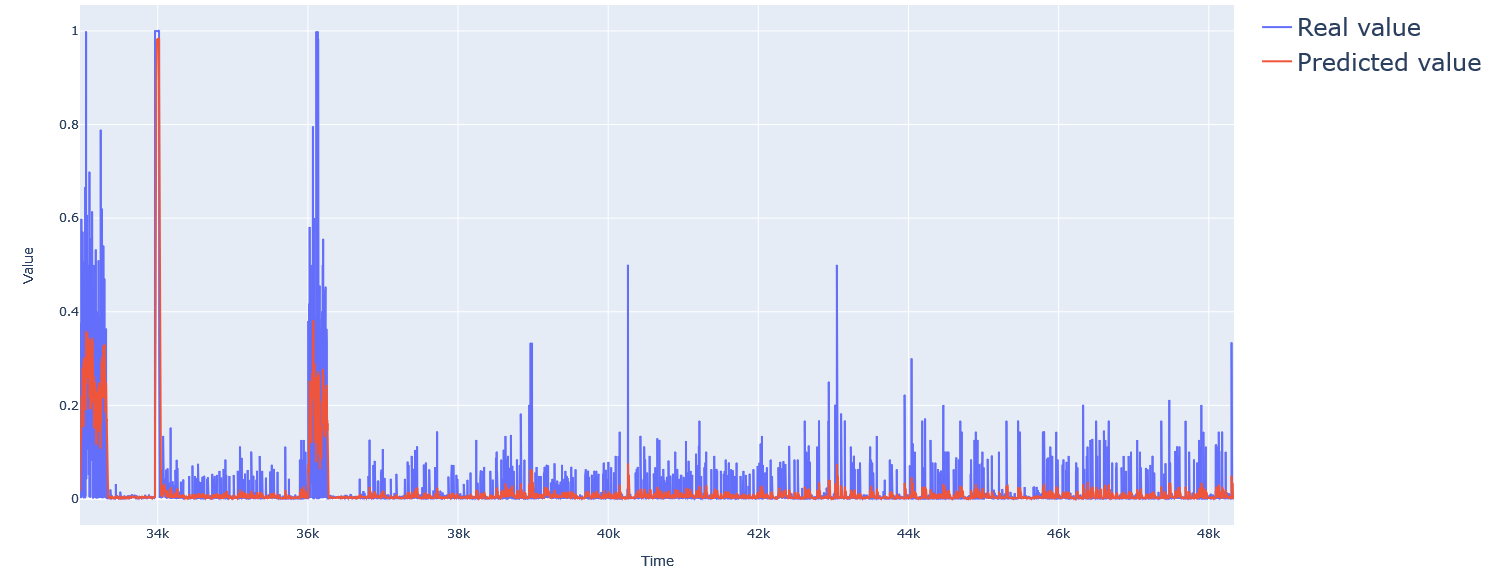
\includegraphics[width=0.7\textwidth]{./input/chapters/models/figs/arma-sol.png}
        \caption{Confronto della previsione del modello e le osservazioni originali sull'insieme di test.}
        \label{fig:arma-sol}
    \end{figure*}

    È evidente che il modello è in grado di prevedere l'andamento generale della serie temporale per la maggior
    parte del dataset. Tuttavia, in alcune aree, il modello presenta una performance inferiore rispetto ad altre.
    Queste aree saranno cruciali per la classificazione dei punti come anomali o non anomali.

    Sulla base delle previsioni $P$, sono stati calcolati i residui rispetto al test set $P-G$ e valutati come punti 
    anomali quelli che soddisfano $p_i-g_i \notin [c^-, c^+] | p_i \in P, g_i \in G$. I residui sono illustrati nella \hyperref[fig:residuals]{Figura 3.3.}

    I punti all'interno dell'intervallo definito dai confini inferiore e superiore non sono considerati anomali. 
    Tra questi punti ci sono quelli blu, che non sono anomalie e che il modello non ha considerato come tali
    (True Negatives), e quelli viola, che il modello ha erroneamente classificato come non anomalie (False Negatives).

    Possiamo inoltre osservare che svariati punti in verde sono sono stati correttamente classificati come anomalie
    (True Positives), ma sono presenti anche molti punti rossi, ovvero quelli che il modello ha erroneamente 
    considerato anomalie (False Positives). 

    \begin{figure}[H]
        \centering
        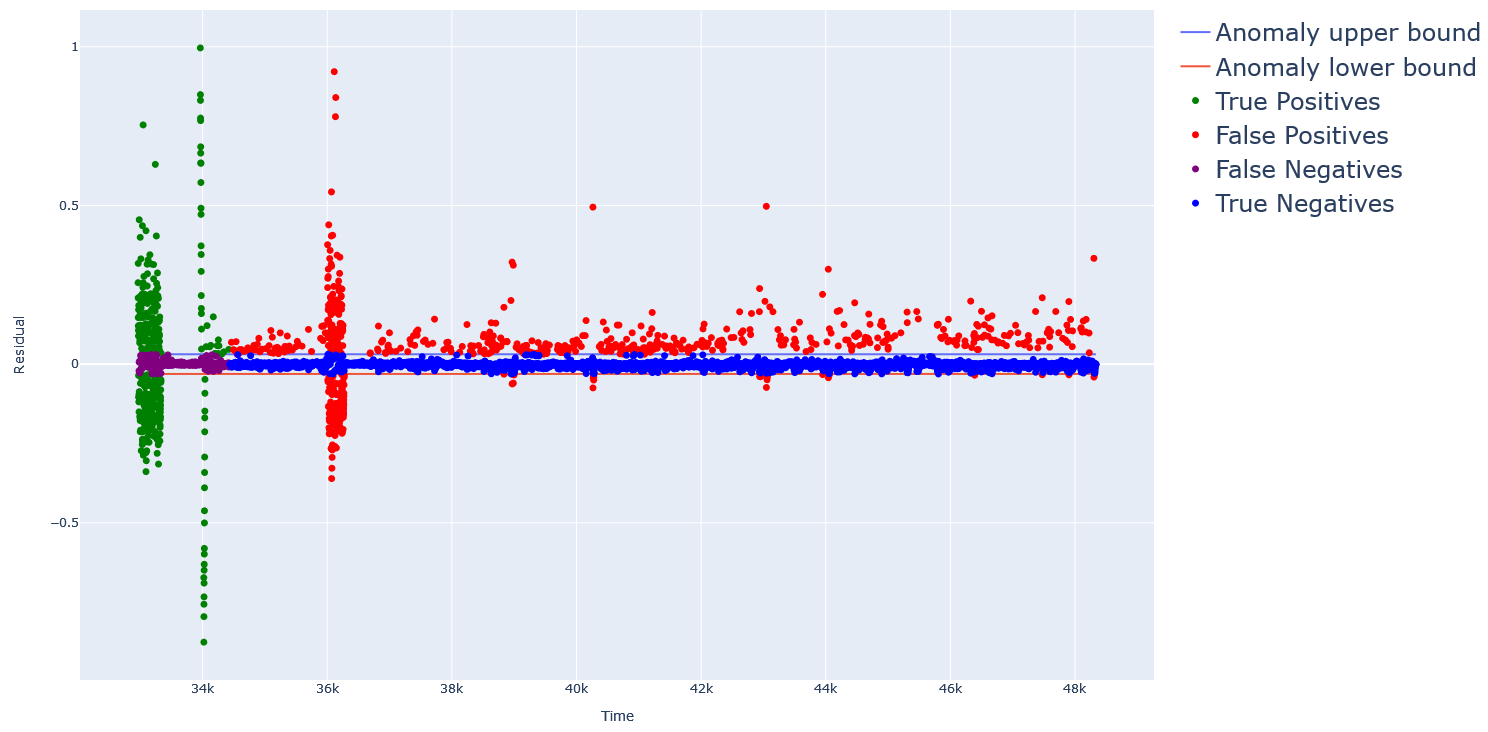
\includegraphics[width=0.7\textwidth]{./input/chapters/models/figs/arma-residuals.png}
        \caption{I residui del modello ARMA nel test set con i confini decisionali che discriminano la previsione delle 
        anomalie e le non anomalie.}
        \label{fig:residuals}
    \end{figure}

    \section{Approccio di Apprendimento Automatico (Machine Learning-based)}
        %**************************************************************
% ocsvm
%**************************************************************
\subsection{One-Class Support Vector Machine}
    In questa sottosezione, esaminiamo il modello basato sull'apprendimento automatico One-Class Support Vector 
    Machine\cite{ocsvm} (OC-SVM) come altro punto di riferimento per valutare le prestazioni del modello 
    MSCRED\cite{mscred}. La scelta del modello OC-SVM è motivata dalla sua ampia utilizzazione nella 
    letteratura di riferimento e dal suo impiego da parte dei ricercatori di MSCRED per il confronto delle 
    prestazioni. In generale, gli algoritmi di tipologia Support Vector Machine sono noti per offrire buone 
    prestazioni in diversi contesti. Tuttavia, tendono a soffrire quando si tratta di classificazione di 
    anomalie, poiché le anomalie costituiscono solitamente una piccola parte del dataset, creando uno 
    sbilanciamento tra le classi.

    \paragraph{Intuizione} OC-SVM, come gli altri algoritmi della famiglia SVM, opera tracciando confini 
    decisionali tra i dati. Nell'ambito della rilevazione delle anomalie, questo si traduce nella definizione 
    di un iperpiano che separa i punti considerati anomali da quelli considerati non anomali.

    \paragraph{Dataset} Nell'esperimento è stato suddiviso il dataset di riferimento negli insiemi di training, 
    validation e test con le stesse percentuali utilizzate per ARMA, ovvero $0.5, 0.182, 0.318$ rispettivamente. 
    La \hyperref[tab:dataset-ocsvm]{Tabella 3.2.} mostra la percentuale di anomalie in ciascun 
    sottoinsieme del dataset originale, mentre nella \hyperref[fig:dataset-div1]{Figura 3.4.} viene
    evidenziato il dataset partizionato.


    \begin{table}[H]
        \centering
        \caption{Statistiche dataset OC-SVM.}
        \begin{tabular}{lccc}
            \toprule
            \textbf{Dataset} & \textbf{Indice di suddivisione} & \textbf{\# punti} & \textbf{Anomalie (\%)} \\
            \toprule
            \textbf{Training}   & 0.5   &  24168 & 2.01\% \\
            \textbf{Validation} & 0.182 &  8797  & 8.60\% \\
            \textbf{Testing}    & 0.318 &  15372 & 9.59\% \\
            \bottomrule
        \end{tabular}
        \label{tab:dataset-ocsvm}
    \end{table}

    \begin{figure}[H]
        \centering
        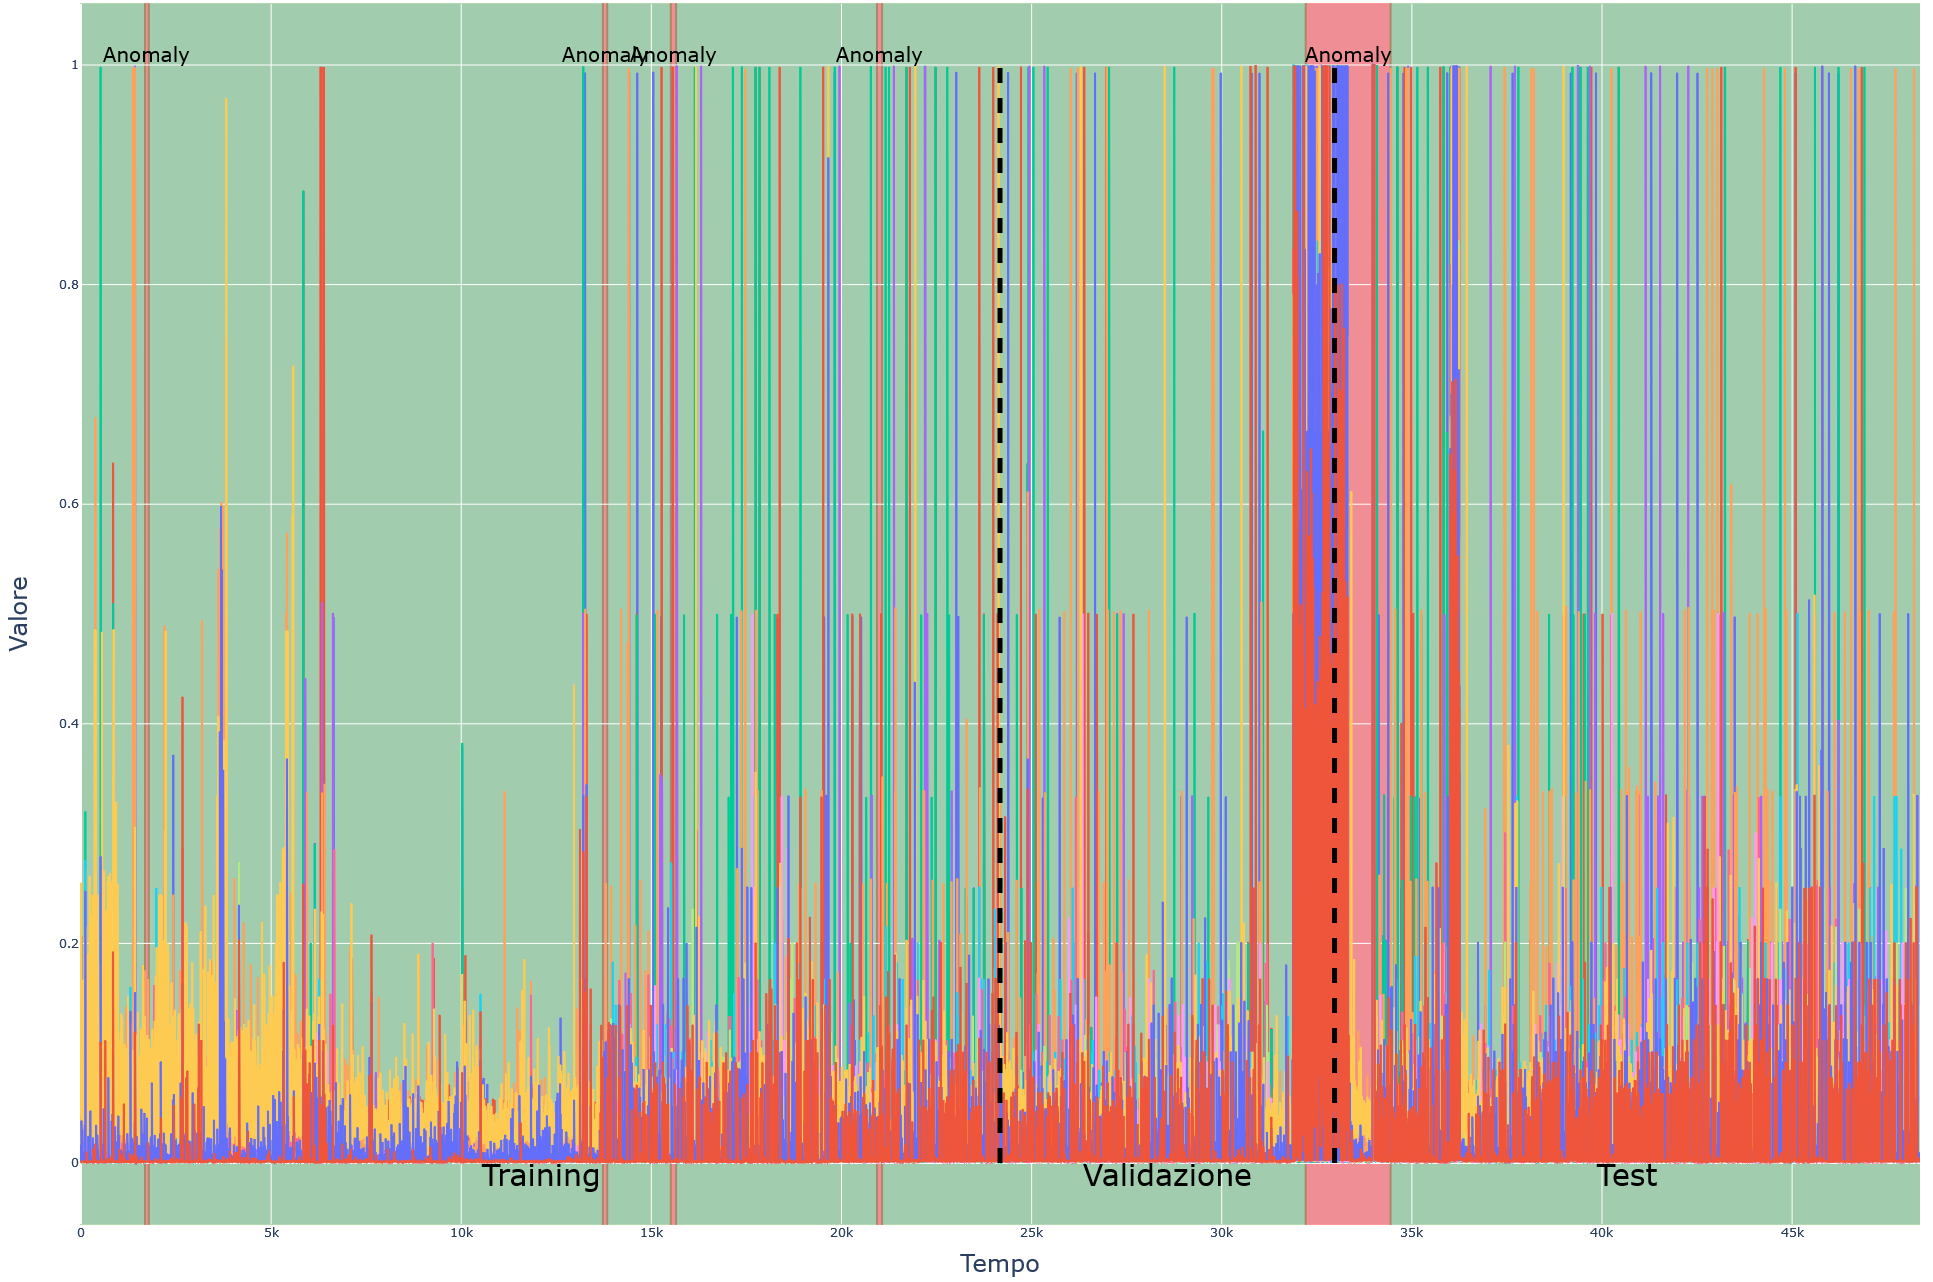
\includegraphics[width=0.5\textwidth]{./input/chapters/models/figs/dataset_div1.png}
        \caption{Suddivisione dataset negli insiemi di training, validation e test. Le due linee 
        tratteggiate rappresentano, da sinistra a destra rispettivamente la suddivisione tra l'insieme di training e 
        validazione e tra l'insieme di validazione e test.}
        \label{fig:dataset-div1}
    \end{figure}


    \begin{table}[H]
        \centering
        \caption{Valori candidati per gli iperparametri.}
        \begin{tabular}{lccc}
            \toprule
            \textbf{Iperparametro} & \textbf{Candidati} \\
            \toprule
            $\nu$ & 0.03, 0.1, 0.25, 0.5, 0.9 \\
            \midrule
            Kernel & linear, poly, rbf, sigmoid \\
            \bottomrule
        \end{tabular}
        \label{tab:iperparametri-candidati}
    \end{table}

        \paragraph{Iperparametri} Gli iperparametri $\nu$ e il tipo di kernel sono stati trovati effettuando una 
        "grid-search" partendo 
        da un insieme di candidati per entrambi gli iperparametri illustrati nella 
        \hyperref[tab:iperparametri-candidati]{Tabella 3.3.} La combinazione di valori $(\nu^*, \text{Kernel}^*)$ che 
        ha massimizzato lo score F1 sul validation set è stata scelta come configurazione ottimale.

        Formalmente, siano $\mathbf{Tr}, \mathbf{Va}$ i dataset utilizzati per il training e
        per il validation rispettivamente e sia $\text{OC-SVM}_\mathbf{X}^\mathbf{Y}$ un modello OC-SVM addestrato
        su $\mathbf{X}$ che effettua previsioni sulle etichette dei punti $\mathbf{Y}$ e sia $K$ l'insieme dei 
        possibili valori che può assumere il kernel, ossia $K=\{\text{linear}, \text{poly}, \text{rbf}, \text{sigmoid}\}$:


    \begin{equation}
        \label{eq:ocsvm-problem}
        \begin{aligned}
            & \nu^*, \text{Kernel}^* = \max_{\nu, \text{Kernel}} F1(\text{OC-SVM}_\mathbf{Tr}^\mathbf{Va}(\nu, \text{Kernel})) \\
            & \text{con il vincolo} \quad \nu \in [0.03, 0.1, 0.25, 0.5, 0.9], \text{Kernel} \in K
        \end{aligned}
    \end{equation}
        
        \paragraph{Soluzione} \hyperref[eq:ocsvm-problem]{L'equazione 3.2}  è stata soddisfatta dai seguenti valori:
        \begin{itemize}
            \item $\nu^* = 0.9$
            \item Kernel$^* = \text{sigmoid}$
        \end{itemize}

        Dopo aver utilizzato l'insieme di validazione esclusivamente per l'ottimizzazione degli iperparametri, 
        è stato poi unito al dataset di addestramento. Successivamente, il modello è stato addestrato sul nuovo
        dataset combinato, utilizzando gli iperparametri che hanno prodotto una soluzione ottimale durante la fase di 
        convalida. In \hyperref[fig:ocsvm-sol]{Figura 3.5.} viene mostrata la 
        soluzione dopo l'applicazione di PCA per fornire una rappresentazione ai primi tre componenti principali.
        
        \begin{figure}[H]
            \centering
            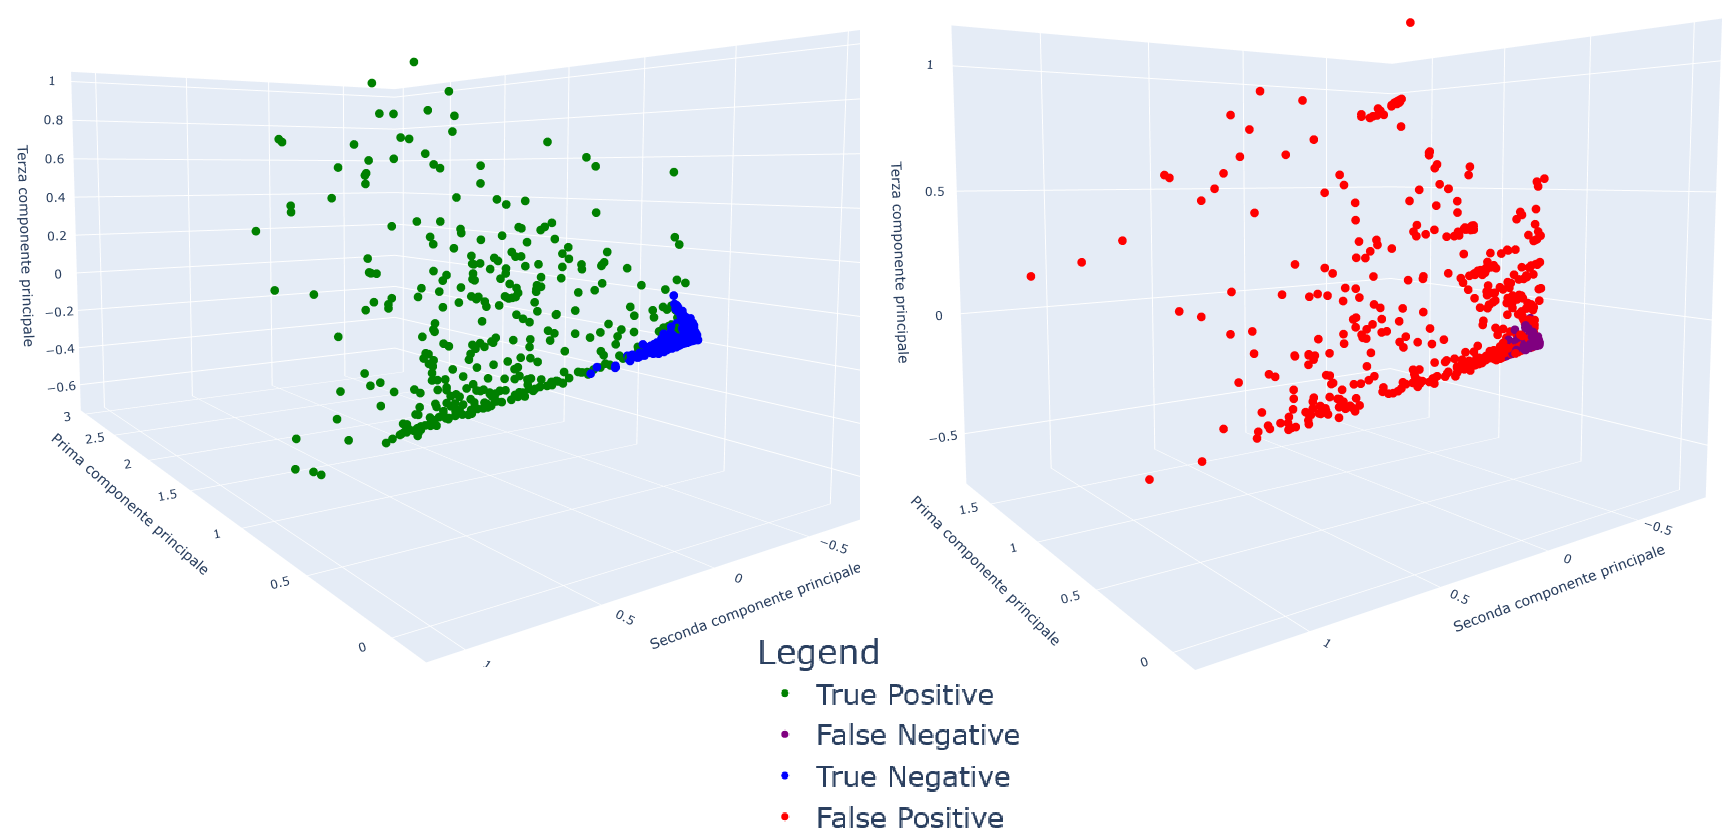
\includegraphics[width=0.7\textwidth]{./input/chapters/models/figs/ocsvm-sol.png}
            \caption{\small
                Soluzione del modello OC-SVM dopo l'applicazione di PCA ai primi tre 
                componenti principali, garantendo una rappresentazione visibile rispetto a quella 
                originale a dodici dimensioni. A sinistra sono rappresentate le previsioni corrette
                (TP, TN), mentre a destra quelle errate (FP, FN).
            }
            \label{fig:ocsvm-sol}
        \end{figure}

        I risultati mostrano chiaramente che il modello ha prestazioni scarse sul dataset di test. 
        I punti verdi a sinistra della \hyperref[fig:ocsvm-sol]{Figura 3.5.} sono quelli classificati correttamente 
        come anomalie (True Positives) e quelli blu sono quelli classificati correttamente come non anomali (True Negatives). 
        Tuttavia, molti punti sono stati classificati in modo errato, come evidenziato a destra nella stessa figura. 
        I punti viola rappresentano le anomalie erroneamente classificate come normali (False Negatives), 
        mentre i punti rossi sono i punti normali erroneamente classificati come anomalie (False Positives).  
        


    \section{Approccio di Apprendimento Profondo (Deep Learning-based)}
          %**************************************************************
% Telemanom
%**************************************************************

\subsection{Telemanom} \label{sez-telemanom}
    Telemanom\cite{telemanom} è una tecnica di rilevazione di anomalie sviluppata dai ricercatori della Nasa nel 2018 
    ai fini dell'anomaly detection su stazioni e veicoli spaziali. Il modello è stato applicato dai ricercatori sui 
    dati telemetrici dei satelliti e del rover Curiosity e, come MSCRED\cite{mscred}, utilizza reti neurali 
    Long-Short Term Memory (LSTM\cite{convlstm}).

    La scelta di utilizzare Telemanom in questa ricerca si è basata sulla necessità di confrontare MSCRED con un modello 
    più recente che sfrutta tecniche avanzate focalizzate sull'apprendimento profondo, concentrandosi esclusivamente 
    sulla rilevazione delle anomalie.

    Il modello nasce come miglioramento ai vecchi sistemi di anomaly detection per l'attrezzatura spaziale 
    che, in generale, erano semplicemente basati su valori precisi e predeterminati che, una volta superati, facevano sì che venissero
    attivate le misure di sicurezza opportune. Telemanom è stato progettato tenendo presente che i dati vivono in un 
    contesto non supervisionato ed è in grado di osservare segnali multipli e analizzare se un certo canale (segnale)
    si trova in uno stato anomalo o meno individualmente dagli altri segnali. Questo permette di tracciare più facilmente 
    le cause dell'anomalia. Per cui Telemanom tratta un contesto ancora più complesso rispetto a quello in cui vive InfoSapienza, 
    dove le anomalie sono globali per tutti i segnali.

    \paragraph{Intuizione} Telemanom effettua previsioni creando un modello distinto per ciascun canale di telemetria,
    questo significa che ogni canale viene trattato in modo indipendente per la previsione. Il modello
    viene addestrato per predire un certo numero di valori futuri per ciascun canale di telemetria. Durante il 
    processo di previsione, l'errore attuale di previsione $e(t) = y(t) - \hat{y}(t)$, in cui $y(t)$ è il valore 
    ground-truth mentre $\hat{y}(t)$ è il valore previsto dal modello, viene smussato attraverso una media 
    ponderata esponenziale. L'insieme degli errori smussati forma un vettore $\mathbf{e}_s$. 
    
    Dato il vettore $\mathbf{e}_s$, la soglia di anomalia è calcolata attraverso un approccio che identifica i valori estremi 
    senza supposizioni sulla distribuzione degli errori. 
    Il threshold $\epsilon$ è calcolato come segue: 
    $\epsilon = \mu(\mathbf{e}_s) + \mathbf{z}\sigma(\mathbf{e}_s)$ in cui $\mathbf{z}$ è una lista ordinata di valori 
    positivi che rappresentano il numero di deviazioni standard sopra la media $\mu(\mathbf{e}_s)$. 

    Sia il vettore $\mathbf{e}_{seq}$ che rappresenta gli errori smussati i cui valori $e^{(i)} \geq \epsilon$, 
    ovvero è un vettore che contiene tutti gli errori smussati che hanno il proprio valore maggiore al valore di threshold, la severità 
    dell'anomalia $s^{(i)}$ per ogni punto è calcolata come segue:

    \[s^{(i)} = \frac{\max(\mathbf{e}_{seq}^{(i)}) - \arg \max(\epsilon)}{\mu(\mathbf{e}_s) + \sigma(\mathbf{e}_s)}\]

    Il rilevamento di anomalie basato sulla previsione dipende in modo significativo dai dati storici utilizzati
    per calcolare la soglia dinamicamente e valutare gli errori di previsione correnti. Da ciò deduciamo che la 
    mancanza di dati storici può portare a falsi positivi che sono calcolati anomali solo a causa del contesto ristretto 
    in cui essi vengono valutati. Telemanom risolve questo problema applicando una procedura di pruning atta a mitigare 
    i falsi positivi e assume che le anomalie di dimensione simile di solito non si verificano frequentemente 
    nello stesso canale. Queste accortezze aiutano a migliorare la precisione del modello, contribuendo a considerare
    i comportamenti normali ma rari delle attrezzature spaziali che si verificano a intervalli regolari.

    \paragraph{Dataset} Telemanom, come già enunciato, prende in considerazione un unico canale alla volta. È 
    quindi necessario suddividere il dataset di Infostud in più parti, una per ogni segnale, per far sì che il modello 
    venga addestrato ed effettui previsioni su tutto il dataset. Gli intervalli anomali associati a ogni canale sono gli 
    stessi, poiché nel caso di InfoSapienza quando avviene un'anomalia, essa è globale per tutti i servizi, quindi 
    per tutti i segnali.

    Per l'esperimento è stato utilizzato lo stesso dataset applicato ai modelli precedenti e discusso nel 
    \hyperref[cap2]{Capitolo 2}, ma il cui indice di split è diverso rispetto ai modelli 
    precedentemente analizzati. Questo perché Telemanom, in generale, prevede un'anomalia se il modello osserva come anomalo 
    l'intervallo in cui l'anomalia si verifica. Le varie metriche, nell'implementazione originale che è stata 
    utilizzata per gli esperimenti, vengono quindi basate solo sugli intervalli considerati anomali, non sul numero 
    di punti previsti come anomali come nelle altre applicazioni analizzate. Il dataset di Infostud preso in 
    analisi ha complessivamente cinque intervalli di anomalie distinte e, se prendessimo 
    in considerazione lo split analizzato precedentemente, solo uno sarebbe nell'insieme di test. Per far sì che il modello 
    sia addestrato e testato in maniera più egregia, è stato scelto lo split osservabile nella 
    \hyperref[tab:dataset-telemanom]{Tabella 3.4.} Il dataset suddiviso è illustrato nella \hyperref[fig:telemanom-data]{Figura 3.6.}, 
    mentre la \hyperref[fig:telemanom-train]{Figura 3.7.} mostra il dataset di addestramento della metrica che 
    rappresenta la latenza media delle richieste di login a InfoSapienza.

    \begin{table}[H]
        \centering
        \caption{Statistiche dataset Telemanom.}
        \begin{tabular}{lccc}
            \toprule
            \textbf{Dataset} & \textbf{Indice di split} & \textbf{\# punti} & \textbf{\# Intervalli anomali} \\
            \midrule
            \textbf{Training} & 0.43 & 20784  & $3$ \\
            \textbf{Testing} & 0.67 & 27553 & $2$ \\
            \bottomrule
        \end{tabular}
        \label{tab:dataset-telemanom}
    \end{table}

    \begin{figure}[H]
        \centering
        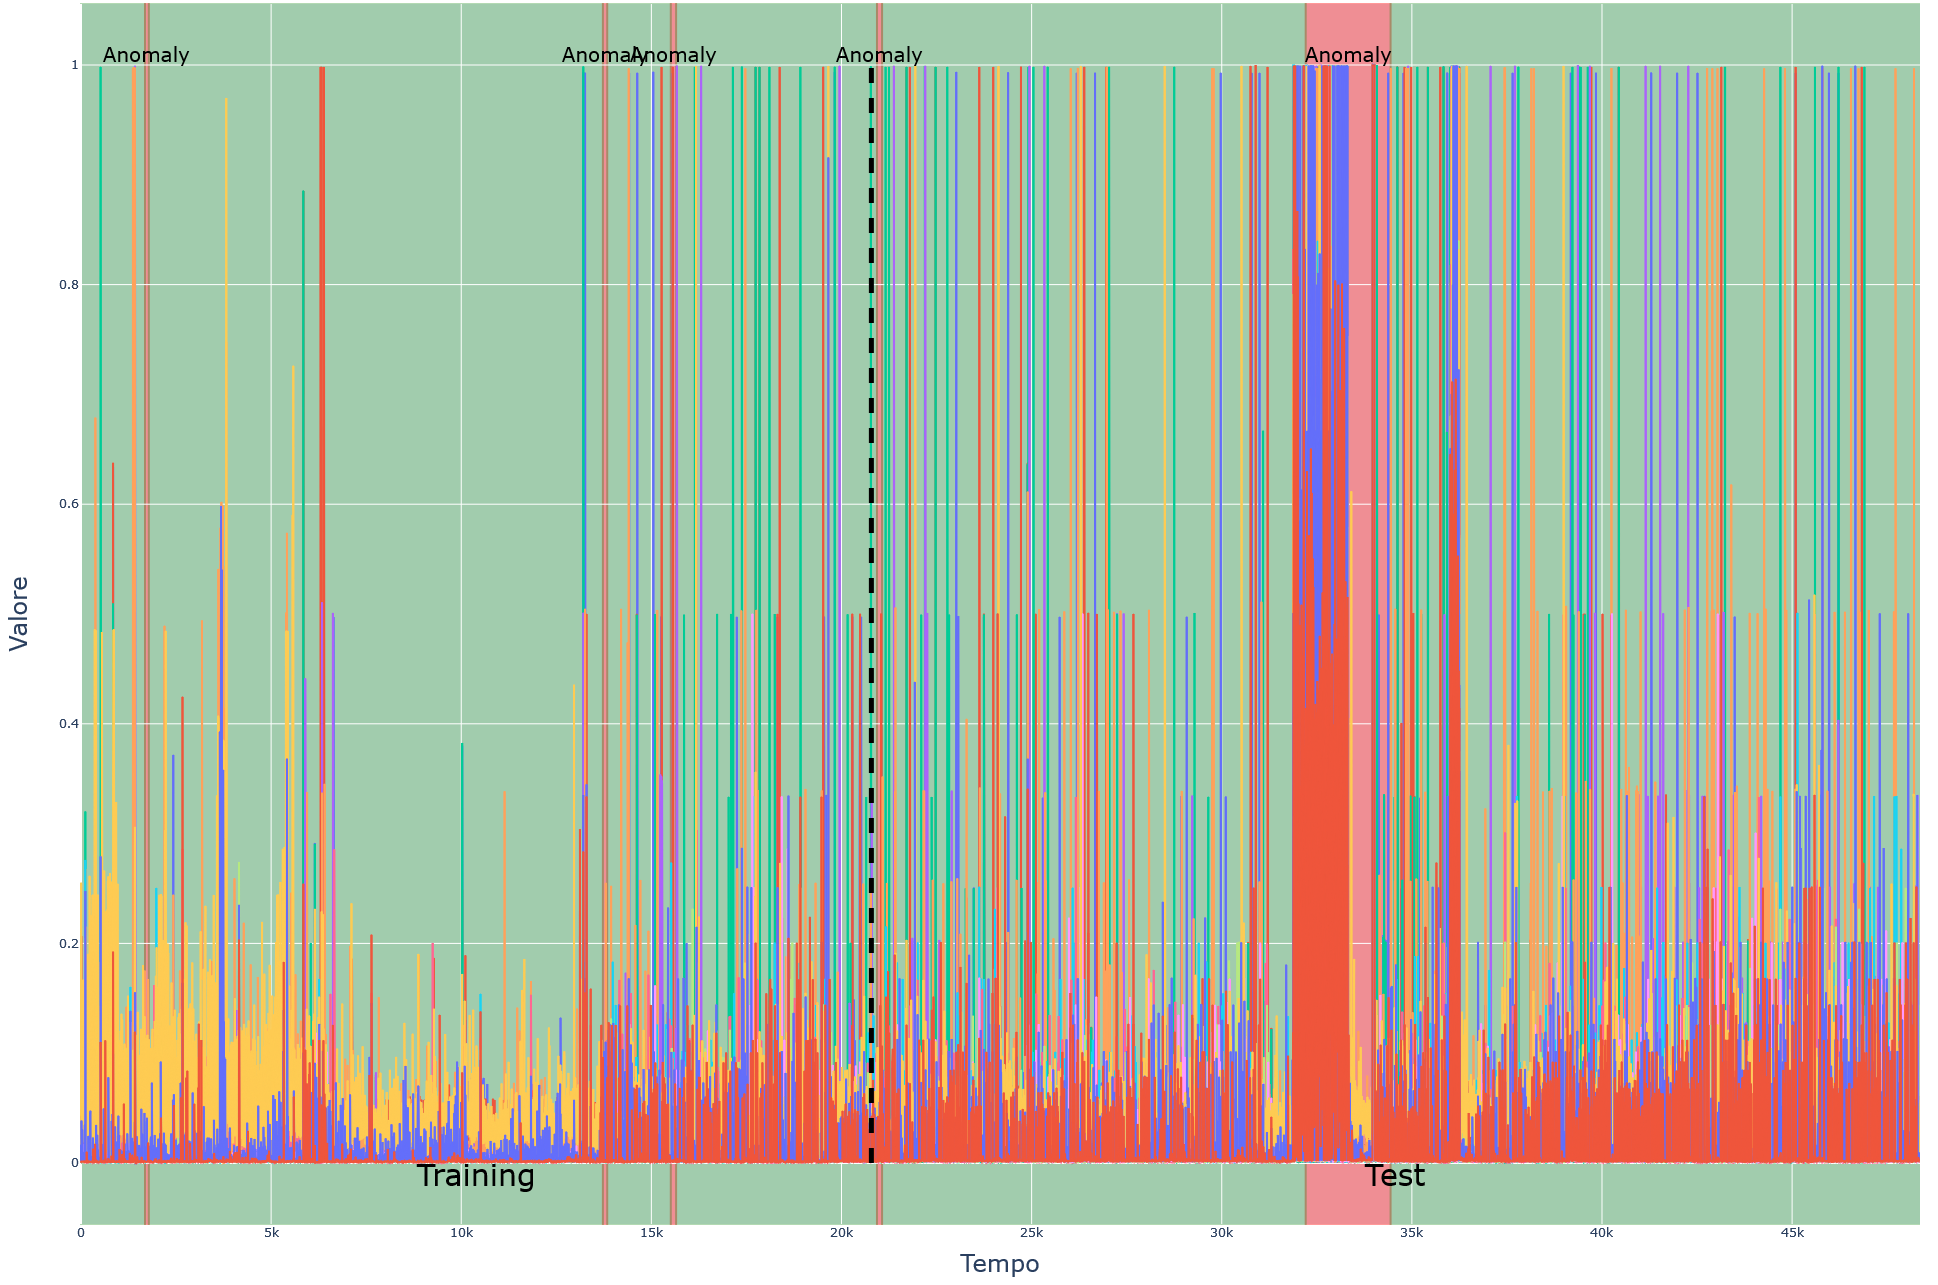
\includegraphics[width=0.6\textwidth]{./input/chapters/models/figs/telemanom-data.png}
        \caption{Suddivisione dataset negli insiemi di training e test. La linea tratteggiata delimita il dataset 
        di training da quello dedicato al test.}
        \label{fig:telemanom-data}
    \end{figure}

    \begin{figure}[H]
        \centering
        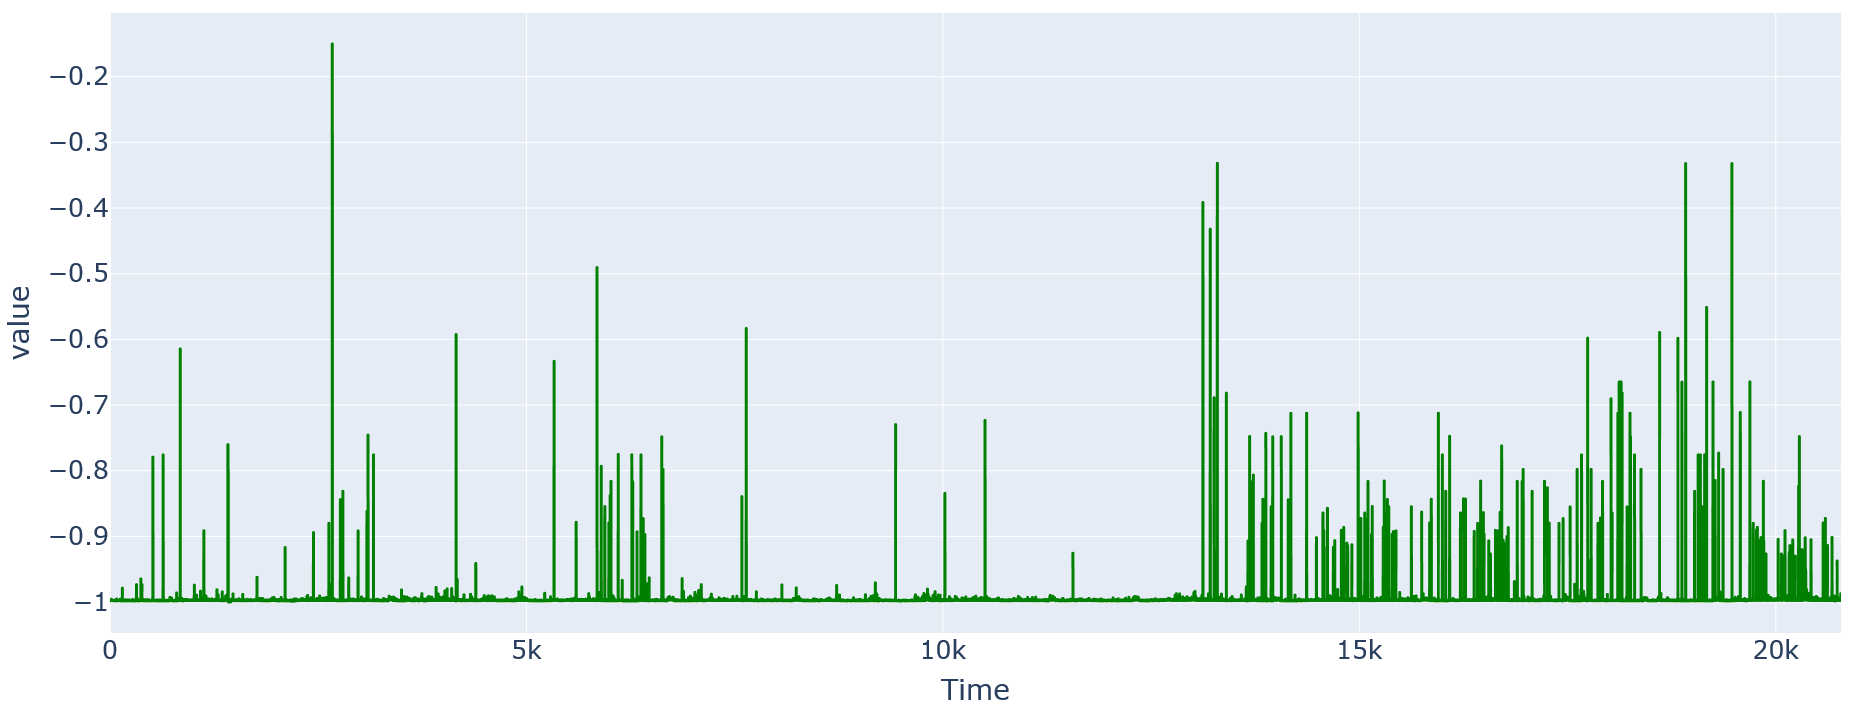
\includegraphics[width=0.7\textwidth]{./input/chapters/models/figs/telemanom-train-data.png}
        \caption{Insieme di training di Telemanom.}
        \label{fig:telemanom-train}
    \end{figure}

    Non è stato necessario assicurare una parte di dati al validation set perché Telemanom, nella sua 
    implementazione, gestisce da sé la validazione per l'addestramento della sua rete neurale.

    \paragraph{Iperparametri} Telemanom presenta numerosi iperparametri, tra i quali i più significativi sono riportati nella
    \hyperref[tab:telemanom-hyperparams]{Tabella 3.5.}, insieme ai valori empiricamente scelti per questo esperimento.
        
    \begin{table}[H]
        \centering
        \caption{Descrizione e valori degli iperparametri Telemanom.}
        \begin{tabular}{p{0.25\linewidth}p{0.55\linewidth}p{0.10\linewidth}}
            \toprule
            \textbf{Iperparametro} & \textbf{Informazioni} & \textbf{Valore}\\
            \toprule
            $batch\_size$ & Indica il numero di valori da considerare in ogni batch durante l'addestramento. & $100$\\
            \midrule
            $window\_size$ & Specifica il numero di batch precedenti da utilizzare nel calcolo dell'errore smussato.  & $110$\\
            \midrule
            $smoothing\_perch$ & Determina l'indice di smussamento nel calcolo degli errori. & $0.1$ \\
            \midrule
            $layers$ & Vettore bidimensionale che rappresenta il numero di neuroni negli strati nascosti della rete neurale. & $[100,100]$\\
            \midrule
            $l_s$ & Numero di passi temporali precedenti a quello attuale su cui verrà basata la previsione futura. & $7$ \\
            \midrule
            $n\_predictions$ & Indica il numero di valori futuri da prevedere. & $35$ \\
            \midrule
            $validation\_split$ & Specifica la percentuale del dataset di training che verrà usato come validazione per l'addestramento 
                della rete neurale. & $0.2$\\
            \bottomrule
        \end{tabular}
        \label{tab:telemanom-hyperparams}
    \end{table}


        % !TEX root = ../thesis.tex
    
%**************************************************************
% MSCRED
%**************************************************************

\subsection{Multi-Scale Convolutional Recurrent Encoder-Decoder}
    MSCRED\cite{mscred} è un recente modello avanzato che si concentra sull'identificazione di anomalie all'interno di serie 
    temporali multivariate.

    \paragraph{Scelta del modello} MSCRED è stato scelto per diverse ragioni; come attestano gli autori del paper,
    è in grado di catturare informazioni a diverse scale temporali, grazie all'incorporazione di strati convoluzionali. 
    Inoltre, la sua architettura di codifica-decodifica è adatta per l'identificazione di pattern complessi. Fondamentalmente, 
    il modello è stato sviluppato con l'obiettivo specifico di gestire l'intercorrelazione dei segnali e la 
    dipendenza temporale tra di essi. Lo scopo principale è valutare se questo approccio avanzato possa migliorare 
    significativamente il rilevamento delle anomalie rispetto a modelli più tradizionali come 
    ARMA\cite{arma} e OC-SVM\cite{ocsvm}.
    
    
    \paragraph{Le controversie sul modello} L'implementazione originale, disponibile su 
    GitHub\footnote{\url{https://github.com/7fantasysz/MSCRED}}, non è stata accolta con entusiasmo dalla critica online. 
    Purtroppo, di per sé, il codice non è molto intuibile e sono presenti 
    dei riferimenti agli ambienti locali dello sviluppatore originale. Inoltre, nell'implementazione originale, le etichette
    che rappresentano le anomalie nel dataset non sono state fornite, rendendo impossibile replicare i risultati del paper.
    Tutto questo ha fatto suscitare dubbi riguardo all'effettiva efficacia del modello. Nella repository 
    GitHub\footnote{\url{https://github.com/Pikarz/tirocinio\_infostud}} relativa agli studi affrontati in questa relazione viene 
    allegata la versione del codice revisionata e rinnovata a fondo dal sottoscritto con cui sono stati effettuati gli esperimenti.


    \paragraph{Il framework del modello}
    Per quanto riguarda il modello in sé, le "signature matrices" sono una parte fondamentale di MSCRED e svolgono un 
    ruolo chiave nell'analisi delle serie temporali. Queste matrici sono utilizzate per rappresentare le intercorrelazioni
    tra diverse coppie di serie temporali in un segmento specifico della serie, una proprietà critica che riflette lo
    stato del sistema.
    

    Le signature matrices sono matrici $n \times n$ dove $n$ è il numero di segnali della serie temporale analizzata.
    Una certa signature matrix $M^t$ è costruita attraverso il prodotto interno di due serie temporali all'interno del segmento 
    interessato. Formalmente, date due serie temporali $\mathbf{x}^w_i = (x^{t-w}_i, x^{t-w-1}_i, \dots, x_i^t)$ e $\mathbf{x}_j^w =
    (x_j^{t-w}, x_j^{t-w-1}, \dots, x_j^t)$ appartenenti allo stesso segmento $X^w$, la loro correlazione $m_{ij}^t \in M^t$ è 
    calcolata secondo l'\hyperref[eq:sign-matr]{equazione 3.3.}

    \begin{equation}\label{eq:sign-matr}
        m_{ij}^t =\frac{\sum_{\delta=0}^w x_i^{t-\delta}x_j^{t-\delta}}{w}
    \end{equation}
            
    \begin{figure}[H]
        \centering
        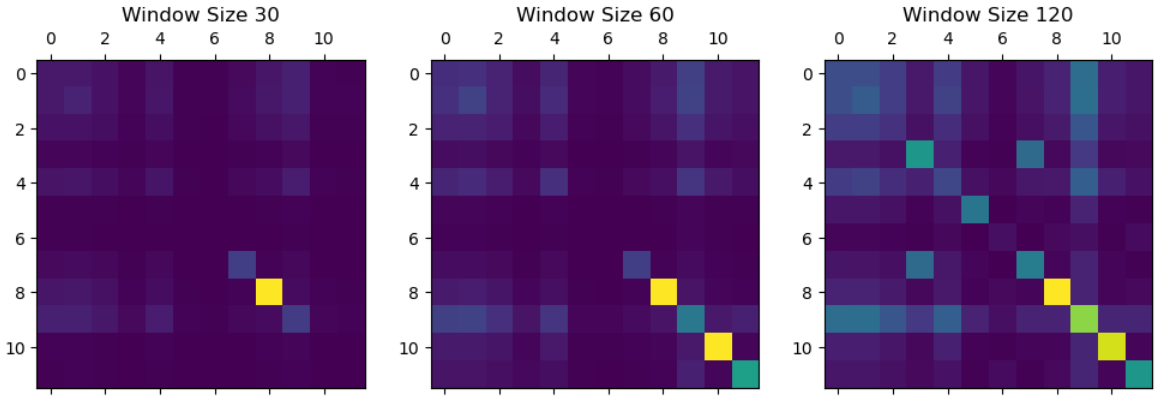
\includegraphics[width=0.6\textwidth]{./input/chapters/models/figs/signature_matrices.png}
        \caption{Signature matrices.} % Use caption to create a caption
        \label{fig:signature-matrices}
    \end{figure}

    Banalmente, le signature matrices sono matrici simmetriche. Nell'esperimento, l'intervallo tra due segmenti è 
    $gap\_time = 30$ e vengono costruite $s=3$ signature matrices con grandezze diverse pari a $win\_sizes = [30, 60, 120]$ punti
    temporali.
    Nella \hyperref[fig:signature-matrices]{Figura 3.8.} è illustrato un esempio di tre signature matrices su cui si
    basano i risultati dell'esperimento riportati nella \hyperref[val-mscred]{Sezione 4.5}.

    In sintesi, le signature matrices vengono concatenate e il tensore risultante $\chi^{t,0} \in \mathbb{R}^{n \times n \times s}$ 
    viene fornito in input a vari strati convoluzionali. Sia $\chi^{t,l}$ la feature map del livello $l$-esimo, attraverso un 
    attention based ConvLSTM\cite{convlstm} vengono aggiornati gli strati nascosti delle feature map $\mathcal{H}^{t,l}$ in $\hat{\mathcal{H}}^{t,l}$. 
    In seguito, attraverso un decodificatore convoluzionale, le feature map ottenute al passo precedente vengono decodificate e
    vengono ricostruite le signature matrices facendo, essenzialmente, il processo inverso: la feature map $\hat{\mathcal{H}}^{t,l}$ 
    viene data in input a una rete neurale deconvoluzionale e l'output, la feature map $\hat{\chi}^{t,l}$, è concatenato 
    con l'output del precedente layer convoluzionale. La concatenazione è poi data in input al prossimo strato deconvoluzionale. 
    L'output finale $\hat{\chi}^{t,0}$ denota le signature matrices ricostruite. La funzione di loss di MSCRED, osservabile
    nell'\hyperref[eq:mscred-loss]{equazione 3.4}, osserva la differenza tra le signature matrices originali e quelle ricostruite e, 
    nel corso delle epoche di training, punta a minimizzare tale funzione di loss.       

    \begin{equation}\label{eq:mscred-loss}
        \mathcal{L}_{MSCRED} = \sum_t \sum_{c=1}^s \Vert \chi^{t,0}_{:,:,c} - \hat{\chi}^{t,0}_{:,:,c} \Vert^2_F
    \end{equation}



    \paragraph{Il dataset} La suddivisione del dataset negli insiemi di training, validazione e test ha mantenuto 
    gli indici di suddivisione usati nell'esperimento di OC-SVM, osservabile nella 
    \hyperref[tab:dataset-ocsvm]{Tabella 3.2.}

    \paragraph{Iperparametri} MSCRED, come già anticipato nei paragrafi precedenti, presenta diversi iperparametri, tra cui 
    $win\_sizes$ che rappresenta la larghezza delle signature matrices, $gap\_time$, che determina la distanza tra i segmenti 
    della serie temporale, ovvero identifica quanto scorre ogni finestra a ogni passo, e $s$ che è il numero signature matrices. 
    Inoltre, l'iperparametro $step\_max$ rappresenta il numero di feature maps precedenti 
    concatenate dal codificatore convoluzionale e $thred\_b$ e $threshold$ regolano la sensibilità del modello 
    nel determinare le anomalie. In particolare, $thred\_b$ rappresenta un valore di soglia specifico utilizzato 
    dal modello per valutare numericamente l'indice di anomalia degli elementi all'interno dei dati, associando a essi
    un certo punteggio di anomalia. $threshold$, invece, è atto a valutare le prestazioni complessive 
    del modello e stabilisce una soglia oltre la quale i punteggi di anomalia vengono etichettati come anomalie.

    Dopo un'attenta analisi sono stati scelti per l'esperimento gli iperparametri riportati nella 
    \hyperref[tab:mscred-iperparams]{Tabella 3.6.} che hanno garantito la migliore soluzione
    empirica. I restanti iperparametri $thred\_b$ e $threshold$, sono stati ottimizzati tramite una grid-search atta 
    a massimizzare la metrica F1.

    \begin{table}[H]
        \centering
        \caption{Iperparametri MSCRED (parte 1.)}
        \begin{tabular}{lc}
            \toprule
            \textbf{Iperparametro} & \textbf{Valore} \\
            \toprule
            $win\_sizes$ & $30, 60, 120$ \\
            $s$ & $3$ \\
            $step\_max$ & $20$ \\
            $gap\_time$ & $30$ \\
            \bottomrule
        \end{tabular}
        \label{tab:mscred-iperparams}
    \end{table}

    Formalmente, siano $\mathbf{Tr}, \mathbf{Va}$ i dataset utilizzati per il training e
    per il validation rispettivamente, e sia $\text{MSCRED}_\mathbf{X}^\mathbf{Y}$ un modello MSCRED addestrato con gli iperparametri 
    della \hyperref[tab:mscred-iperparams]{Tabella 3.6.} su $\mathbf{X}$ che effettua previsioni nei punti $\mathbf{Y}$, 
    e sia $thred\_bs_{50}$ uno spazio lineare costituito da elementi equidistanti $thred\_b_i$ tali che $thred\_b_i \in 
    [1\mathrm{e}{-11}, 1\mathrm{e}{-6}] \forall i \in [50]$ e sia 
    $Thres$ la lista esaustiva dei possibili threshold, ovvero dei vari anomaly score $V_{\text{score}}$, 
    generati dal modello per ogni punto:

    \begin{equation}
        \label{eq:mscred-problem}
        \begin{aligned}
            & thred\_b^*, threshold^* = \max_{\substack{thred\_b, \\ threshold}} F1(\text{MSCRED}_\mathbf{Tr}^\mathbf{Va}(thred\_b, threshold)) \\
            & \text{con il vincolo} \quad thred\_b \in thred\_bs_{50}, threshold \in V_{\text{score}}
        \end{aligned}
    \end{equation}

    \begin{table}[H]
        \centering
        \caption{Iperparametri MSCRED (parte 2.)}
        \begin{tabular}{lc}
            \toprule
            \textbf{Iperparametro} & \textbf{Valore} \\
            \toprule
            $thred\_b^*$ & $6.326$ \\
            $threshold^*$ & $134.747$ \\
            \bottomrule
        \end{tabular}
        \label{tab:mscred-iperparams2}
    \end{table}
    Gli iperparametri che hanno soddisfatto l'\hyperref[eq:mscred-problem]{equazione 3.5} sono riportati nella 
    \hyperref[tab:mscred-iperparams2]{Tabella 3.7.}

    È bene notare che un numero di passaggi temporali pari a $gap\_time$ vengono collassati in uno singolo dopo la computazione di MSCRED,
    quindi data una serie temporale che contiene $x$ osservazioni, la soluzione generata avrà $x \bmod gap\_time$ osservazioni.
    % !TEX root = ../../../thesis.tex
    
%**************************************************************
% Methodology
%*************************************************************

\chapter{Valutazione}
    In questo capitolo vengono analizzate le metriche di valutazione prese in considerazione ai fini 
    dell'analisi del dataset reale delle richieste a servizi fatte a Infostud, la piattaforma su cui si fonda 
    la carriera accademica di tutti gli affiliati all'università La Sapienza.

    \section{Metriche di Valutazione}
        %**************************************************************
% Metriche di Valutazione
%**************************************************************

Nel contesto dell'analisi condotta sui dati osservati della piattaforma Infostud, è fondamentale valutare numericamente 
le soluzioni dei modelli applicati ai fini della valutazione delle loro performance. A tale scopo, vengono utilizzate 
tre metriche importanti: la precisione (precision), il richiamo (recall) e la F1-score (F1) al fine di misurare 
l'efficacia delle soluzioni in modo rigoroso. Queste metriche sono essenziali per comprendere in modo completo ed 
esaustivo l'efficacia degli approcci metodologici applicati.

\subsection{Precisione (Precision)}\label{precision}
    La precisione è una metrica che misura quanto un modello è accurato nel predire gli esempi positivi, o anomali nel 
    contesto dell'anomaly detection, rispetto a tutti 
    i casi che il modello ha classificato come positivi. 
    Per calcolare la precisione, viene valutata la frazione di predizioni positive fatte dal modello che sono effettivamente 
    corrette.
    \[Precision = \frac{TP}{TP+FP}\]\
    Dove:
    \begin{enumerate}
        \item TP (True Positives) rappresenta il numero di casi positivi, o anomali,
        correttamente classificati dal modello.
        \item FP (False Positives) sono i casi negativi erroneamente classificati come positivi, o anomali, dal modello.
    \end{enumerate}
    La precisione fornisce un riscontro numerico che, se massimizzato, rende il modello affidabile quando afferma 
    che un caso è positivo. Tuttavia, la precisione da sola potrebbe non fornire una visione completa delle prestazioni 
    di un modello.

\subsection{Richiamo (Recall)}
    Il richiamo misura la capacità di un modello di individuare tutti gli esempi positivi correttamente. In altre parole, 
    indica quanto il modello fornisce soluzioni che correttamente identificano gli esempi positivi. Il richiamo 
    viene calcolato attraverso la frazione di predizioni positive, o anomale, fatte 
    dal modello rispetto al totale dei casi positivi effettivi.
    \[Recall = \frac{TP}{TP+FN}\]
    Dove:
    \begin{enumerate}
        \item TP sono i True Positives, definiti nella \hyperref[precision]{Sottosezione 4.1.1}
        \item FN (False Negatives) rappresenta il numero di casi positivi, o anomali, erroneamente classificati come negativi 
              dal modello.
    \end{enumerate}
    Un alto valore di richiamo indica che il modello ha un'ottima capacità di individuare gli esempi positivi, ma 
    non tiene in considerazione il numero di casi falsi positivi.

\subsection{F1-Score (F1)}\label{f1-score}
    L'F1-score è una metrica che combina la precisione e il richiamo in un valore che tiene conto sia dei falsi positivi 
    che dei falsi negativi. La metrica bilancia la precisione e il richiamo. La formula per calcolare l'F1-score è 
    la seguente:
    \[F1 = \frac{2\cdot Precision \cdot Recall}{Precision+Recall}\]
    L'F1-score, quindi, mira a cercare un compromesso tra i valori di precisione e richiamo.



    \section{Valutazione del modello statistico ARMA}
        %**************************************************************
% Valutazione ARMA
%**************************************************************

Come è stato già osservato, il modello statistico ARMA racchiude in modo discreto il comportamento del dataset e indica come anomalie i casi in 
cui la previsione del modello si discosta molto dai dati reali. In particolare, gli iperparametri scelti 
hanno riportato uno score F1 di 0.750 sul dataset di validation, mentre 
le metriche osservate sull'insieme di test sono riportate nella \hyperref[tab:arma-metrics]{Tabella 4.1.}

\begin{table}[H]
    \centering
    \caption{Risultati ARMA.}
    \begin{tabular}{lr}
    \toprule
    \textbf{Soluzione ARMA sul test set}  \\
    \midrule
    \multirow{3}{*}{\textbf{Metriche}} & Precisione: 0.332 \\
    & Recall: 0.248 \\
    & F1-score: 0.284 \\
    \bottomrule
    \end{tabular}
    \label{tab:arma-metrics}
\end{table}

I risultati mostrano che ARMA riesce a catturare la tendenza generale del modello e molti 
andamenti anomali vengono predetti come tali. La soluzione non è ottimale, ma fornisce 
comunque una buona base per la valutazione di MSCRED.

    \section{Valutazione del modello ML OC-SVM}
        %**************************************************************
% Valutazione OC-SVM
%**************************************************************

Il metodo che si basa sul machine learning, One-Class Support Vector Machine, arricchisce l'analisi e lo studio 
delle anomalie sul daset di Infostud fornendo una soluzione molto buona sull'insieme di validazione con uno score F1 pari 
a 0.716, e una discreta sull'insieme di test, come mostrato nella 
\hyperref[tab:ocsvm-metrics]{Figura 4.2.}


\begin{table}[H]
    \centering
    \caption{Soluzione OC-SVM.}
    \begin{tabular}{lr}
    \toprule
    \textbf{Soluzione OC-SVM sul test set}  \\
    \midrule
    \multirow{3}{*}{\textbf{Metriche}} 
        & Precisione: 0.331 \\
        & Recall: 0.290 \\
        & F1-score: 0.309 \\
    \bottomrule
    \end{tabular}
    \label{tab:ocsvm-metrics}
\end{table}

I risultati mostrano che OC-SVM è in grado di produrre buoni risultati durante la fase di 
validazione ma fallisce durante la fase di test. Tuttavia, è importante notare che il modello è stato applicato 
in un contesto avverso, caratterizzato da un forte sbilanciamento tra le classi. Nonostante l'ambiente sfavorevole, 
questa soluzione è un punto di riferimento ragionevole per valutare le prestazioni del modello MSCRED.

    \section{Valutazione del modello DL Telemanom}
        %**************************************************************
% Valutazione Telemanom
%**************************************************************

Gli iperparametri ottimali applicati al dataset interessato hanno generato una buona soluzione come evidenziato nella
    \hyperref[tab:telemanom-metrics]{Tabella 4.3.}

    \begin{table}[H]
        \centering
        \caption{Risultati Telemanom.}
        \begin{tabular}{lr}
        \toprule
        \textbf{Soluzione Telemanom sul test set}  \\
        \midrule
        \multirow{3}{*}{\textbf{Metriche}} 
            & Precisione: 1.0 \\
            & Recall: 0.5 \\
            & F1-score: 0.66 \\
        \bottomrule
        \end{tabular}
        \label{tab:telemanom-metrics}
    \end{table}

La soluzione sembra ottima, notevolmente migliore rispetto a quelle dei modelli precedenti, tuttavia non è totalmente 
valida nella nostra applicazione e il motivo è semplice: Telemanom gestisce le anomalie, e calcola metriche su esse,
basandosi solo sugli intervalli anomali come già citato nella \hyperref[sez-telemanom]{Sottosezione 3.3.1}. Gli intervalli anomali ground-truth
nell'esperimento appena riportato sono solo due: uno grande che dura considerevolmente nel tempo, mentre l'altro 
molto più piccolo, come si evince nella \hyperref[fig:telemanom-ys-comparison]{Figura 4.1.}, in cui 
sono illustrati i valori reali e i valori previsti dal modello del dataset che rappresenta la latenza media 
delle richieste di login a Infostud. Telemanom identifica sempre e solo l'intervallo più grande come anomalo 
nei modelli dei vari canali, mentre quello più piccolo non è mai rilevato. Ciò ha portato a una soluzione che
sembra ottima, ma che in realtà, per struttura stessa del modello e dei dati che osserva, sta overfittando il 
dataset. Nella \hyperref[fig:telemanom-e_s]{Figura 4.2.} viene illustrato il grafico degli errori
smussati $\mathbf{e}_s$ riferente allo stesso segnale precedente.

\begin{figure}[H]
    \centering
    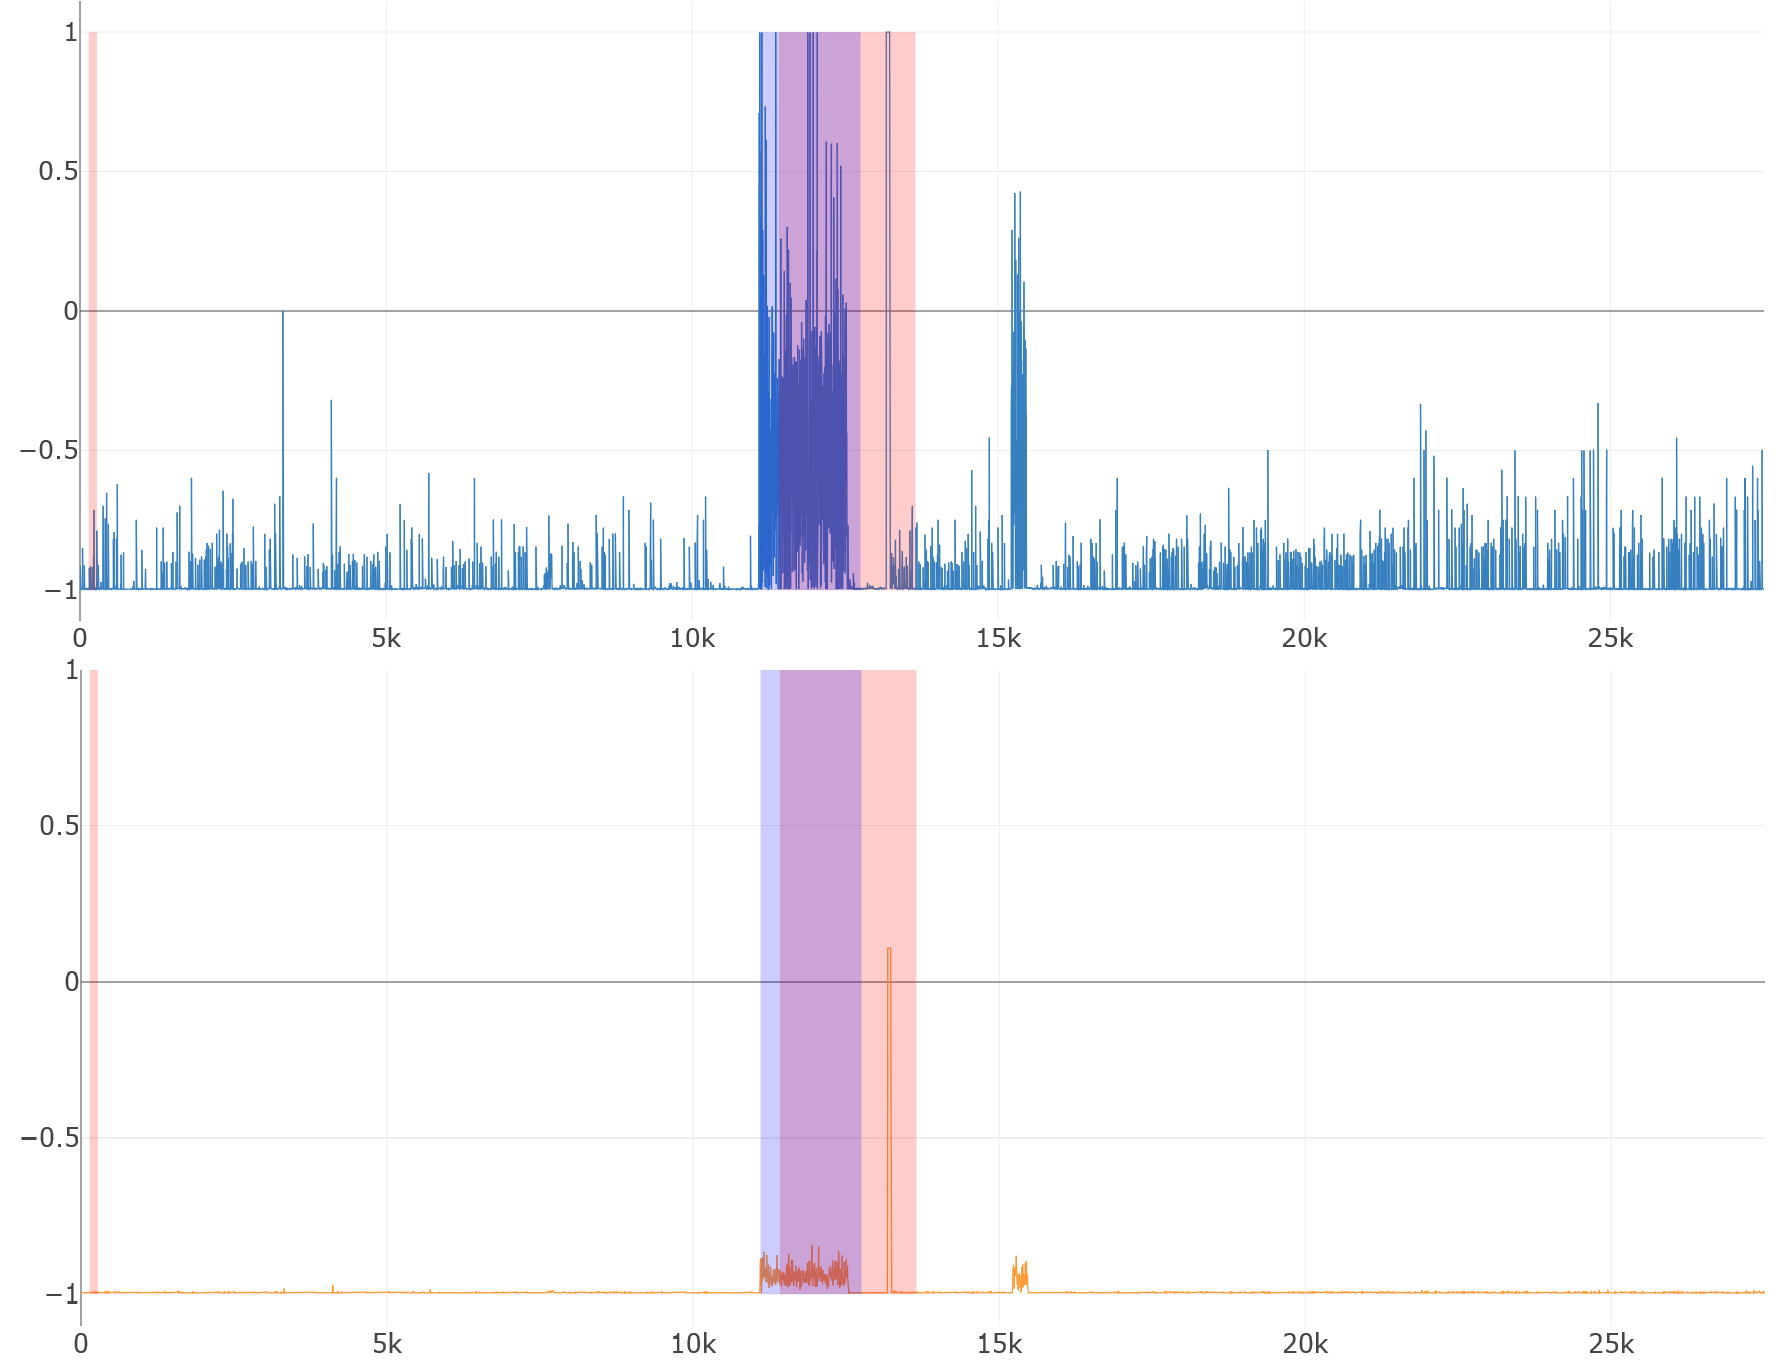
\includegraphics[width=0.7\textwidth]{./input/chapters/models/figs/telemanom-ys-comparison.png}
    \caption{Dati reali $y$ (sopra) e previsione di Telemanom $\hat{y}$ (sotto) della latenza media delle richieste
    login a InfoSapienza. Le bande rosse rappresentano periodi anomali ground-truth, la banda blu è l'intervallo 
    che il modello giudica anomalo.}
    \label{fig:telemanom-ys-comparison}
\end{figure}

\begin{figure}[H]
    \centering
    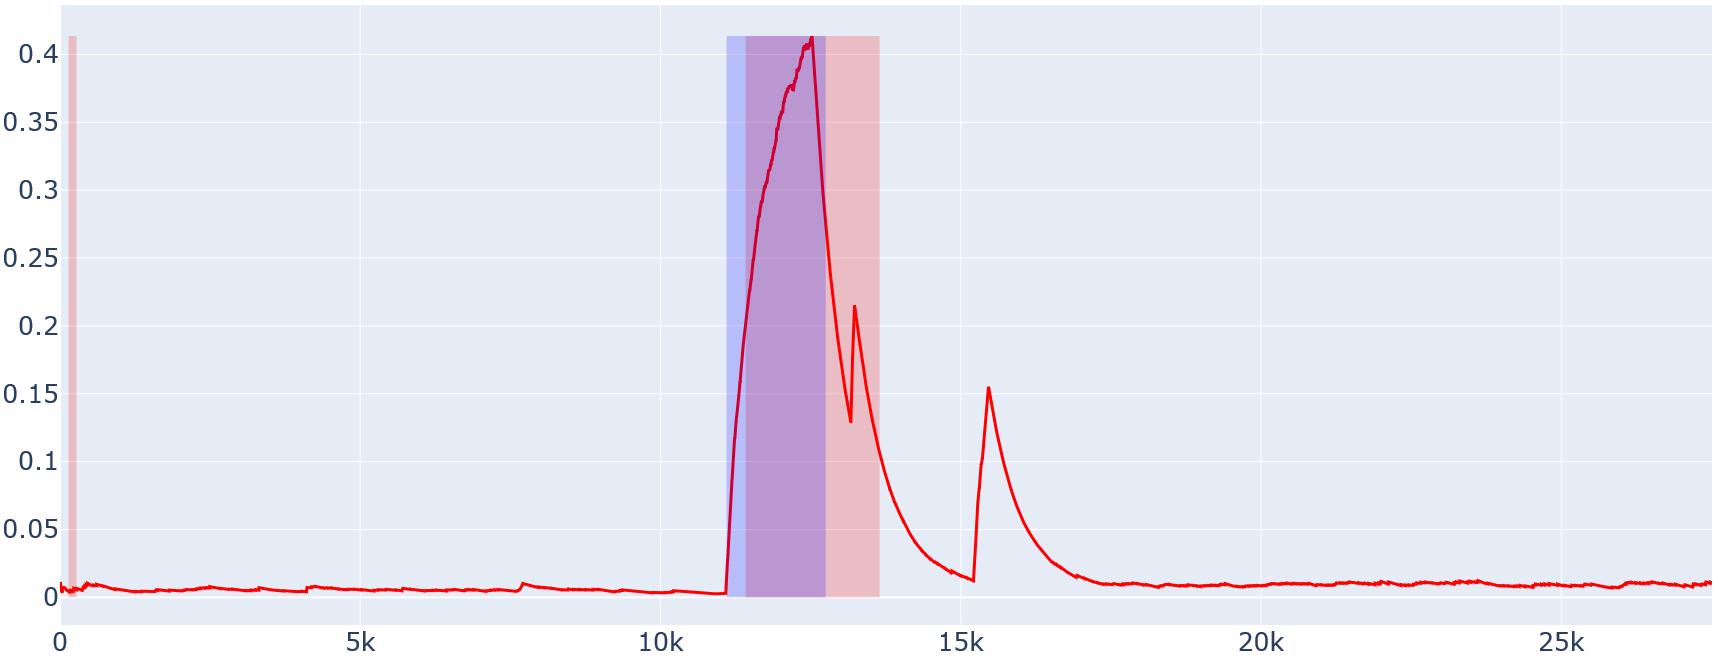
\includegraphics[width=0.7\textwidth]{./input/chapters/models/figs/telemanom-e_s.png}
    \caption{Errore smussato tra i valori reali e la previsione del modello $\mathbf{e}_s$ dei dati che rappresentano la 
    latenza media delle richieste login a InfoSapienza.}
    \label{fig:telemanom-e_s}
\end{figure}


Durante il mio studio di Telemanom ho compreso che il modello, in un contesto in cui sono presenti più anomalie 
che non durano molto nel tempo non performa in maniera altrettanto ottimale. Per riuscire a ottenere un 
discreto punteggio di recall, viene generato un grande numero di falsi positivi; i risultati rimangono coerenti 
a ciò che gli autori originali hanno descritto nel paper: Telemanom, purtroppo, genera molti falsi positivi, e non sembra che 
le sue capacità di pruning, nell'ambito di InfoSapienza, riescano a mitigare molto il problema.
    
In sintesi Telemanom, purtroppo, non si presta bene nel contesto della rilevazione di anomalie 
del dataset di Infostud. Il risultato, seppur ottimo, non viene ritenuto valido perché genera una soluzione che, 
in una situazione più naturale, sarebbe stata molto diversa.
    \section{Valutazione del modello DL MSCRED}
        %**************************************************************
% Valutazione MSCRED
%**************************************************************
\label{val-mscred}
Dopo 7 epoche di addestramento, MSCRED ha proposto la soluzione riportata in \hyperref[fig:sol-valid-mscred]{Figura 4.3.} per l'insieme 
di validazione. Evidenziamo come MSCRED riesca a percepire l'andamento improvvisamente anomalo della serie temporale estratta 
dal dataset di Infostud, 
generando anomaly score elevati per ogni punto corrispondente a uno dei ventisei delle anomalie ground-truth, 
evidenziate dall'area rossa. In questo caso, la soluzione ha portato a un risultato perfetto, ottenendo uno score 
F1 pari a 1.0 e affermando l'ipotesi sollevata nel \hyperref[cap2:hypothesis]{Capitolo 2}: il dataset che rappresenta 
le latenze medie è un ottimo indicatore per quanto riguarda l'analisi e l'individuazione delle anomalie.

Riguardo all'insieme di test, MSCRED ha ottenuto risultati leggermente inferiori ma propone comunque una soluzione ottima 
mostrata in \hyperref[fig:sol-test-mscred]{Figura 4.4.} Le metriche risultanti dalla soluzione sono riportate 
nella \hyperref[tab:mscred-metrics]{Tabella 4.4.}

\begin{figure}[H]
    \centering
    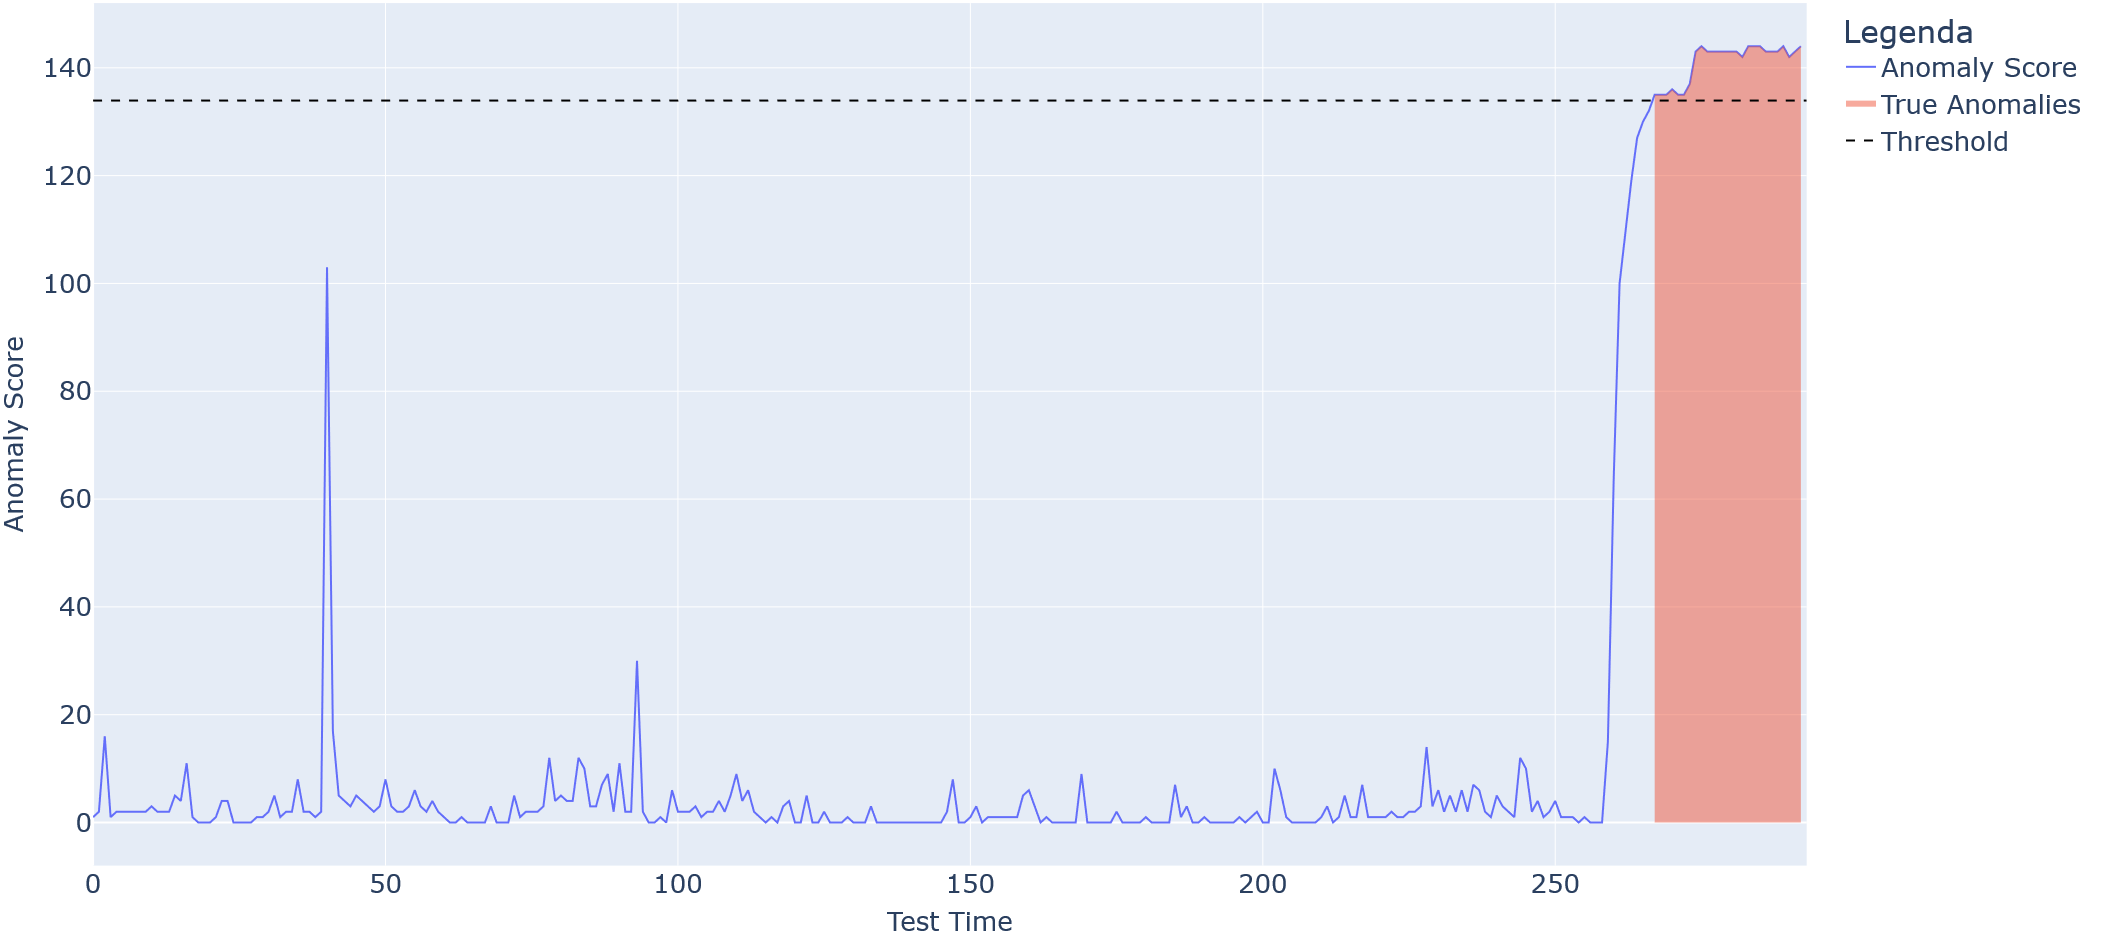
\includegraphics[width=0.7\textwidth]{./input/chapters/models/figs/sol-valid-mscred.png}
    \caption{Soluzione MSCRED sul validation set.}
    \label{fig:sol-valid-mscred}
\end{figure}


\begin{figure}[H]
    \centering
    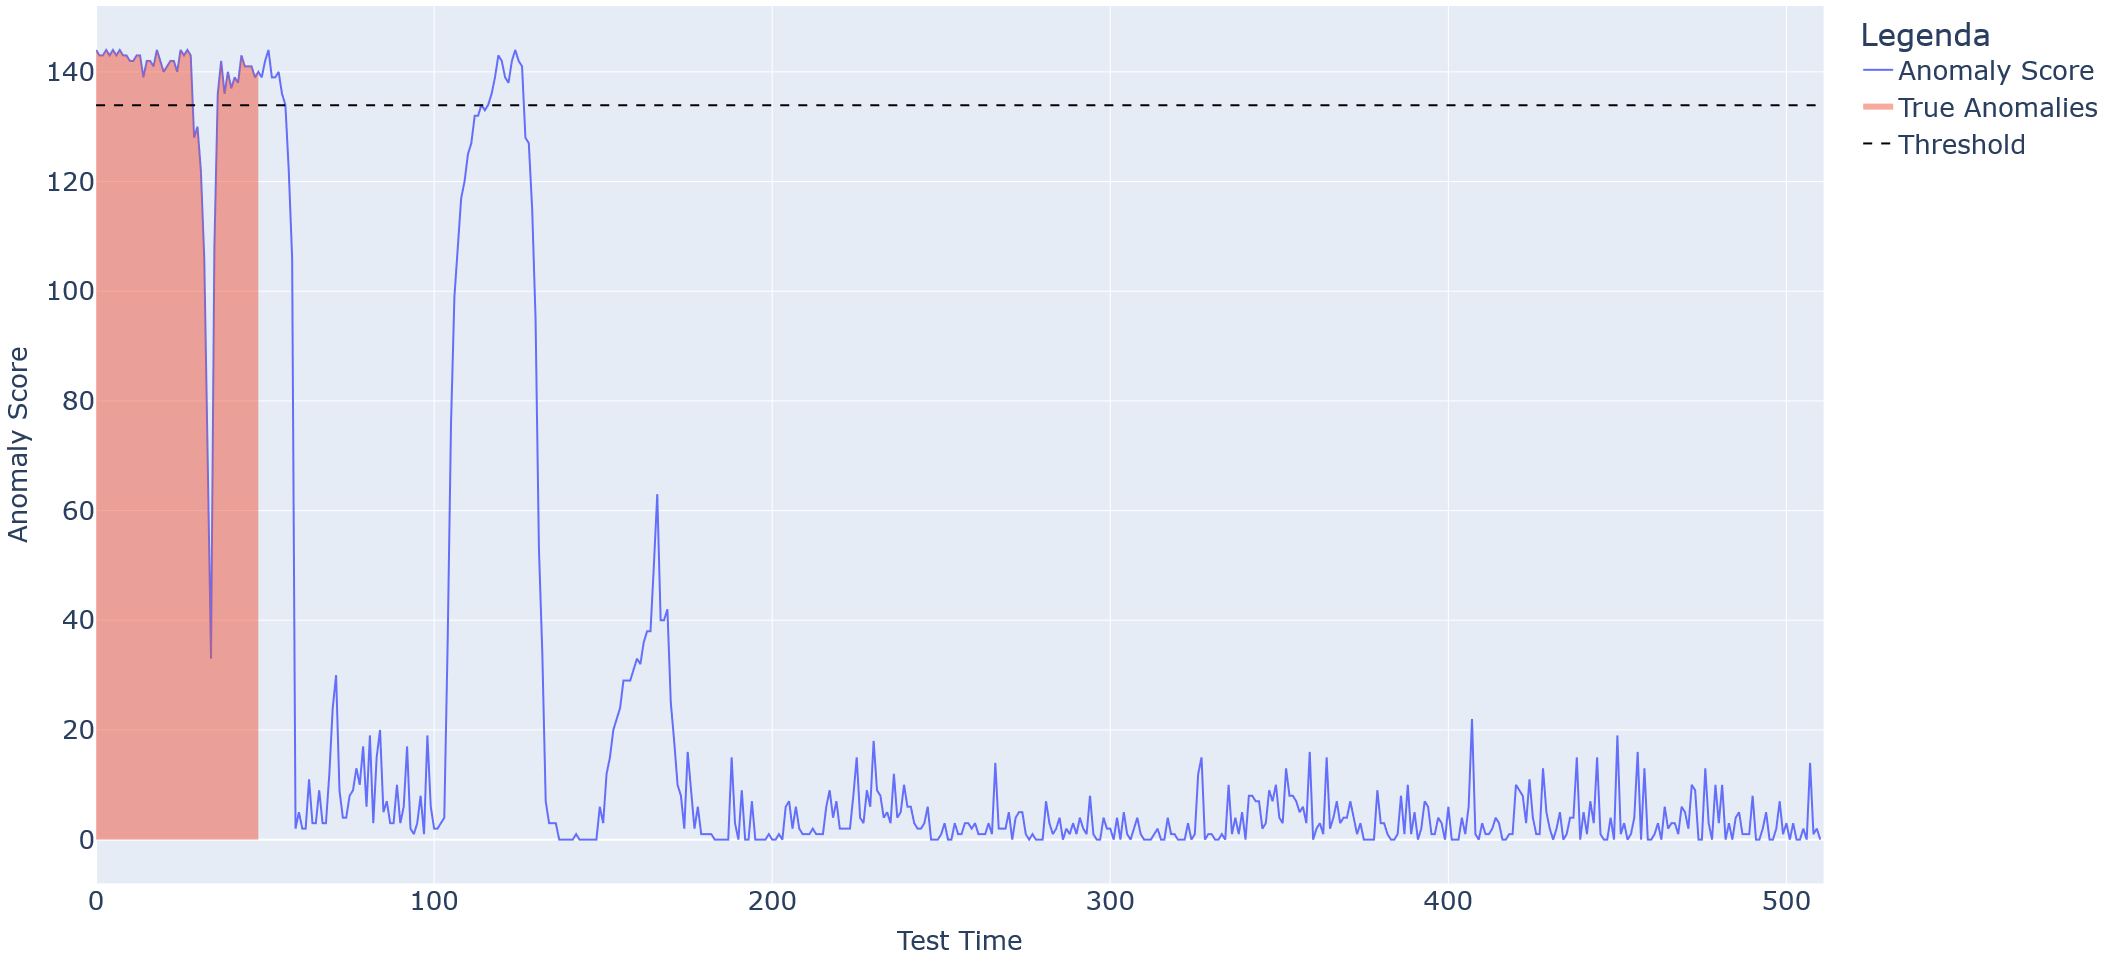
\includegraphics[width=0.7\textwidth]{./input/chapters/models/figs/sol-test-mscred.png}
    \caption{Soluzione MSCRED sul test set.}
    \label{fig:sol-test-mscred}
\end{figure}

\begin{table}[H]
    \centering
    \caption{Risultati MSCRED.}
    \begin{tabular}{lr}
    \toprule
    \textbf{Soluzione MSCRED sul test set}  \\
    \midrule
    \multirow{3}{*}{\textbf{Metriche}} & Precisione: 0.711 \\
    & Recall: 0.857 \\
    & F1-score: 0.777 \\
    \bottomrule
    \end{tabular}
    \label{tab:mscred-metrics}
\end{table}

\paragraph{Conclusioni} I risultati dimostrano in maniera cristallina che MSCRED fornisce
soluzioni notevolmente migliori rispetto agli altri metodi presi in analisi.
Il modello, inoltre, riesce a catturare l'intercorrelazione dei segnali e la dipendenza temporale che
hanno le osservazioni vicine nello spazio, e quindi nel tempo, delle serie temporali multivariate.
MSCRED offre una misura numerica della severità delle anomalie anziché una semplice classificazione binaria, 
soddisfacendo così tutti i requisiti per un algoritmo di rilevamento delle anomalie discussi nel 
\hyperref[cap:intro]{Capitolo 1.} e permettendo all'anomaly detection di compiere un grande passo avanti. 

D'altro canto, però, assumendo che il dataset di Infostud preso in analisi rispetti 
la proprietà IID, MSCRED sembra non offrire soluzioni altrettanto ottimali su serie temporali molto lunghe, ma fa sì che alcune anomalie pesino 
molto più di altre e non garantisce più una netta differenza tra i periodi anomali e non anomali. Questa supposizione 
è basata su delle prove fatte durante il percorso di studio di MSCRED: più è lunga la serie temporale, più 
MSCRED sembra performare in maniera peggiore. Tale affermazione, però, richiede studi più approfonditi per poter 
essere dimostrata o smentita.
    % !TEX root = ../thesis.tex
    
%**************************************************************
% Conclusioni
%**************************************************************

\chapter{Conclusioni: un passo avanti verso soluzioni migliori}
        Nell'ambito degli studi affrontati, sono stati esplorati diversi algoritmi per la rilevazione di anomalie 
        sulla serie temporale multivariata estratta dalla piattaforma indispensabile per tutta la nostra comunità accademica. 
        Gli esperimenti hanno fornito preziose informazioni sulle prestazioni di 
        questi algoritmi e sulle loro potenzialità in questo complesso e affascinante dominio di applicazione; tali soluzioni,
        auspicabilmente, potrebbero essere analizzate per far sì che vi siano miglioramenti sulle operazioni e sul 
        tempo di risposta e di processamento dei servizi richiesti, potenzialmente garantendo un ambiente migliore a tutti 
        coloro che, giornalmente, beneficiano della piattaforma universitaria Infostud. 
        È stato un onore per il sottoscritto poter interagire con dati di tale rilevanza e di così
        stretto coinvolgimento.

        \paragraph{ARMA: il modello consolidato} Nonostante ARMA\cite{arma} (Auto Regressive Moving Average) non sia stato 
        originariamente progettato per il rilevamento di anomalie, rimane un pilastro tra gli algoritmi tradizionali. 
        ARMA è un modello robusto ed efficace, basato su semplici metodi statistici ma adattabile a numerosi contesti della 
        data science, e dimostra solidità anche nella rilevazione di anomalie.

        \paragraph{OC-SVM: una soluzione sfacciata} L'algoritmo dall'approccio metodologico del machine learning visto 
        in questi studi è stato OC-SVM\cite{ocsvm}. Sebbene questo algoritmo fosse molto sfavorito per il contesto
        preso in considerazione, visto l'intrinseco sbilanciamento tra le classi nell'anomaly detection,
        ha comunque offerto una soluzione degna di interesse. OC-SVM è un algoritmo flessibile e ci ha garantito
        un'ottima base su cui misurare le performance future.


        \paragraph{Telemanom: la non-soluzione} Purtroppo Telemanom\cite{telemanom}, nonostante sia un modello molto recente 
        che si focalizza sull'anomaly detection attraverso il deep learning, offre una soluzione che overfitta i dati. 
        L'overfit non è tanto dovuto agli iperparametri, quanto a come il modello gestisce le anomalie e a come 
        esse sono naturalmente distribuite nel dataset preso in analisi. La soluzione di Telemanom, seppur buona numericamente, 
        non è da prendere in considerazione.

        \paragraph{MSCRED: un promettente avanzamento} MSCRED\cite{mscred} (Multi-Scale Convolutional Recurrent Encoder-Decoder) 
        è un modello relativamente giovane che si basa sul deep learning. Le analisi illustrate suggeriscono che MSCRED, grazie 
        alla sua capacità di catturare l'intercorrelazione tra i segnali e la loro dipendenza temporale, emerge come un 
        candidato di spicco per futuri sviluppi nel campo dell'anomaly detection. Il modello ha dimostrato ottime 
        performance senza richiedere un eccessivo tuning degli iperparametri, lasciando intravedere un promettente futuro.

        \paragraph{Riassunto: Le Performance degli Algoritmi} La \hyperref[tab:recap-perf]{Tabella 5.1.} riassume 
        le performance dei vari algoritmi esaminati mediante le metriche principali prese in considerazione.


    \begin{table}[H]
        \centering
        \caption{Performance dei modelli analizzati}
        \begin{tabular}{lcccc}
        \toprule
        \textbf{Modello} & \textbf{Precisione} & \textbf{Recall} & \textbf{F1-score} \\
        \midrule
        \textbf{OC-SVM} & 0.331 & 0.290 & 0.309 \\
        \textbf{ARMA} & 0.332 & 0.248 & 0.284 \\
        \textbf{Telemanom}\footnote{}  & \emph{1.0} & \emph{0.5} & \emph{0.66} \\
        \textbf{MSCRED} & \textbf{0.711} & \textbf{0.857} & \textbf{0.777} \\
        \bottomrule
        \end{tabular}
        \label{tab:recap-perf}
    \end{table}
    
        \footnotetext{La soluzione non è valida perché il modello non è adatto al contesto di InfoSapienza}
        \paragraph{Il futuro dell'anomaly detection} L'obiettivo per il futuro che ci attende è quello di sviluppare 
        soluzioni sempre più accurate, che possano identificare le anomalie nei sistemi complessi attribuendo un valore 
        numerico che identifichi lo stato, anomalo o meno, del sistema. Ciò garantirà non solo la possibilità di prendere atto 
        prontamente delle anomalie, ma renderà possibile anche la loro prevenzione, contribuendo così a migliorare 
        la sicurezza e minimizzando i periodi di down dei sistemi in una varietà di settori industriali, in cui spesso 
        vi è in ballo anche la vita umana.
      % conclusioni

    \backmatter

    \cleardoublepage
    \phantomsection

    % !TEX root = ../thesis.tex
    
%**************************************************************
% Bibliography
%*************************************************************


\begin{thebibliography}{4}

    \bibitem{telemanom}
    Christopher Laporte, Ian Colwell, Kyle Hundman, Tom Soderstrom, Valentino Constantinou\\
    \textit{Telemanom: Detecting Spacecraft Anomalies Using LSTMs and Nonparametric Dynamic Thresholding}.\\
    Disponibile al link \url{https://arxiv.org/abs/1802.04431}, 2018.\\
    arXiv:1802.04431v3 [cs.LG] 6 Jun 2018.

    \bibitem{mscred} 
    Chuxu Zhang, Dongjin Song, Yuncong Chen, Xinyang Feng\\
    \textit{MSCRED: A deep neural network for unsupervised anomaly detection and diagnosis in multivariate time series data}.\\
    Disponibile al link \url{https://dl.acm.org/doi/10.1609/aaai.v33i01.33011409}, 2019.\\
    The Thirty-Third AAAI Conference on Artificial Intelligence (AAAI-19).

    \bibitem{ocsvm}
    Larry M. Manevitz, Malik Yousef\\
    \textit{One-Class SVMs for Document Classification}.\\
    J. Mach. Learn. Res. 2(Dec):139–154.

    \bibitem{arma}
    Peter J. Brockwell, Richard A. Davis\\
    \textit{An Introduction to Time Series and Forecasting}.

    \bibitem{convlstm}
    Xingjian SHI, Zhourong Chen, Hao Wang, Dit-Yan Yeung, Wai-kin Wong, Wang-chun Woo.\\
    \textit{Convolutional LSTM Network: A Machine Learning Approach for Precipitation Nowcasting}.\\
    NIPS, 802–810.
    
\end{thebibliography}                      % bibliografia



\end{document} 